\documentclass[journal]{IEEEtran}
\hyphenation{op-tical net-works semi-conduc-tor}
\usepackage{cite}
\usepackage{graphicx}
\usepackage{amsmath}
\usepackage{amssymb}
\usepackage{multirow}
\usepackage{booktabs}
\usepackage[table]{xcolor}
\usepackage{listings}
\usepackage{footnote}
\usepackage{bm}
\usepackage[normalem]{ulem}
\useunder{\uline}{\ul}{}
\usepackage{amsfonts}
\usepackage{algorithm}
\usepackage{algorithmic}
\usepackage{marvosym}

%%%%%%%%%%%%%%%%%%%%%%%%%%%%%%%%%%%%%%%%%%%%%%%%%%%%%%%%%%%%%%%%%%%%%%%%
%% 投稿前核验标记：
%% 黄底红字 \FILLIN{...} 表示必须由作者用原始 GT、原始预测概率图和正式评测脚本确认。
%% Fig.\ref{ablavis} 原标注的 Full=0.79 / High=0.61 / Low=0.57 无法从排版图稳定复现，
%% 且 High/Low 面板存在疑似错配，因此不得把图像反算值当作正式实验结果。
%%%%%%%%%%%%%%%%%%%%%%%%%%%%%%%%%%%%%%%%%%%%%%%%%%%%%%%%%%%%%%%%%%%%%%%%
\definecolor{fillorange}{RGB}{200,60,0}
\definecolor{fillyellow}{RGB}{255,242,0}
\newcommand{\FILLIN}[1]{\colorbox{fillyellow}{\textcolor{fillorange}{\textbf{[[TO FILL #1]]}}}}

\begin{document}

\title{Harnessing Frequency-Aware Network for Crack Detection in Road-Perceptive Autonomous Vehicle Scenes}


\author{Senyun Kuang, Yintao Wei, Yang Liu, and Xiaobo Qu,~\IEEEmembership{Senior Member,~IEEE}%
\thanks{This work was supported by the National Natural Science Foundation of China [grant numbers 51761135124, 11672148, 52003142, 51775293]; and the State Key Laboratory of Vehicle NVH and Safety Technology [Grant number NVHSKI-202106]. The authors are with the State Key Laboratory of Automotive Safety and Energy, Tsinghua University, Beijing 100084, China. The authors' email addresses are: ksy23@mails.tsinghua.edu.cn, weiyt@tsinghua.edu.cn, xiaobo@tsinghua.edu.cn, and liuy@chalmers.se.}}

\markboth{Submit to IEEE Transactions on Cybernetics}%
{Shell \MakeLowercase{\textit{et al.}}: Bare Demo of IEEEtran.cls for IEEE Journals}

\maketitle


\begin{abstract}
With the evolution of intelligent transportation systems, the integration of crack detection capabilities in vehicles has seen significant advancements. Existing deep-learning-based crack detection methods, predominantly focused on the RGB domain, often fall short in complex scenarios where cracks blend seamlessly with their background. Recognizing that road cracks and surrounding pavement features exhibit greater discriminative potential in the frequency domain, we introduce a novel frequency-aware mechanism. Our frequency-aware network (FANet) operates in two steps: a frequency-guided coarse crack localization step for initial crack identification, followed by a detail-preserving fine crack segmentation step for enhanced precision. Leveraging features from different backbone levels, FANet employs a frequency-aware module for effective coarse localization. Subsequently, a hybrid fusion module integrates high-level features via prior-guided correction and incorporates shallow features to refine crack details. Empirical evaluations on five datasets demonstrate FANet's superior performance.
\end{abstract}

\begin{IEEEkeywords}
Crack Detection, Frequency-aware Feature Learning, Road-perceptive Vehicles
\end{IEEEkeywords}


\section{Introduction}\label{sec1}

Maintaining the structural integrity of infrastructure is paramount, with crack detection playing a crucial role in safeguarding facilities against the detrimental effects of deterioration. Timely detection and remediation of cracks are essential for preventing potentially irreversible damage. The advent of autonomous vehicles and advanced environmental perception technologies~\cite{DBLP:journals/tcyb/HuzaefaL23,DBLP:journals/tcyb/CaoRS23,DBLP:journals/tcyb/ZhangLLGGCL24} heralds a new era in automated road condition monitoring, with autonomous road-perceptive vehicles poised to revolutionize how we maintain our roadways~\cite{9543474,
mohan2018crack,9998084,
DBLP:journals/tcyb/XieWLLLWZJ24,Almaskati2024}. Integrating crack detection capabilities into these vehicles offers a promising pathway for continuous road condition surveillance~\cite{Zhang2024}.

\begin{figure}
\centering
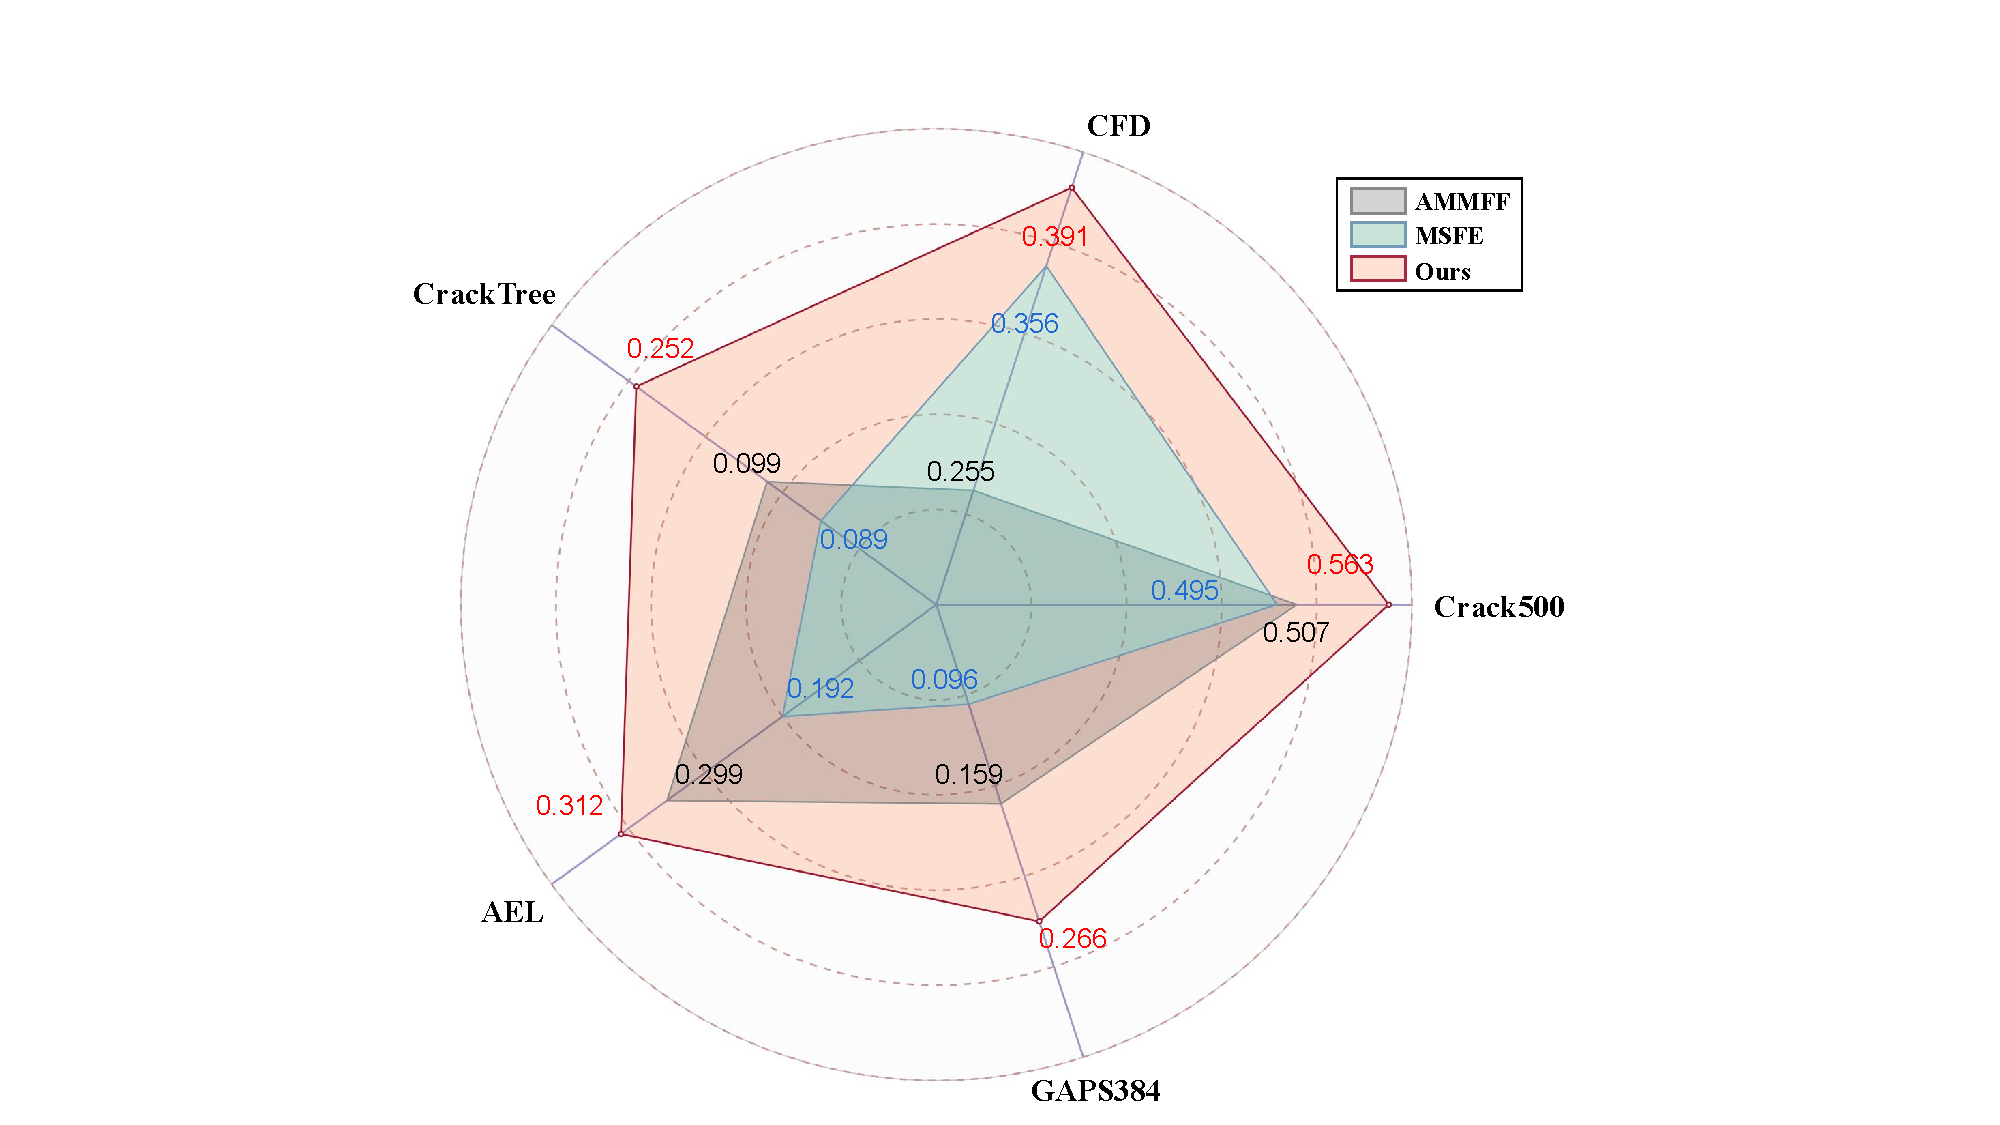
\includegraphics[width=0.83\linewidth]{spider0330.pdf}
\caption{AIU comparison of FANet, AMMFF~\cite{DBLP:journals/tits/QuCWYL22}, and MSFE~\cite{DBLP:journals/tiv/ZhouQJ23} on Crack500~\cite{DBLP:journals/tits/YangZYPML20}, GAPs384~\cite{DBLP:conf/ijcnn/EisenbachSSADSE17}, CrackTree200~\cite{DBLP:journals/prl/ZouCLMW12}, CFD~\cite{DBLP:journals/tits/ShiCQMC16}, and AEL~\cite{DBLP:journals/tits/AmhazCIB16}.}
\label{introdvis}
\end{figure}

\begin{figure*}[!t]
\centering
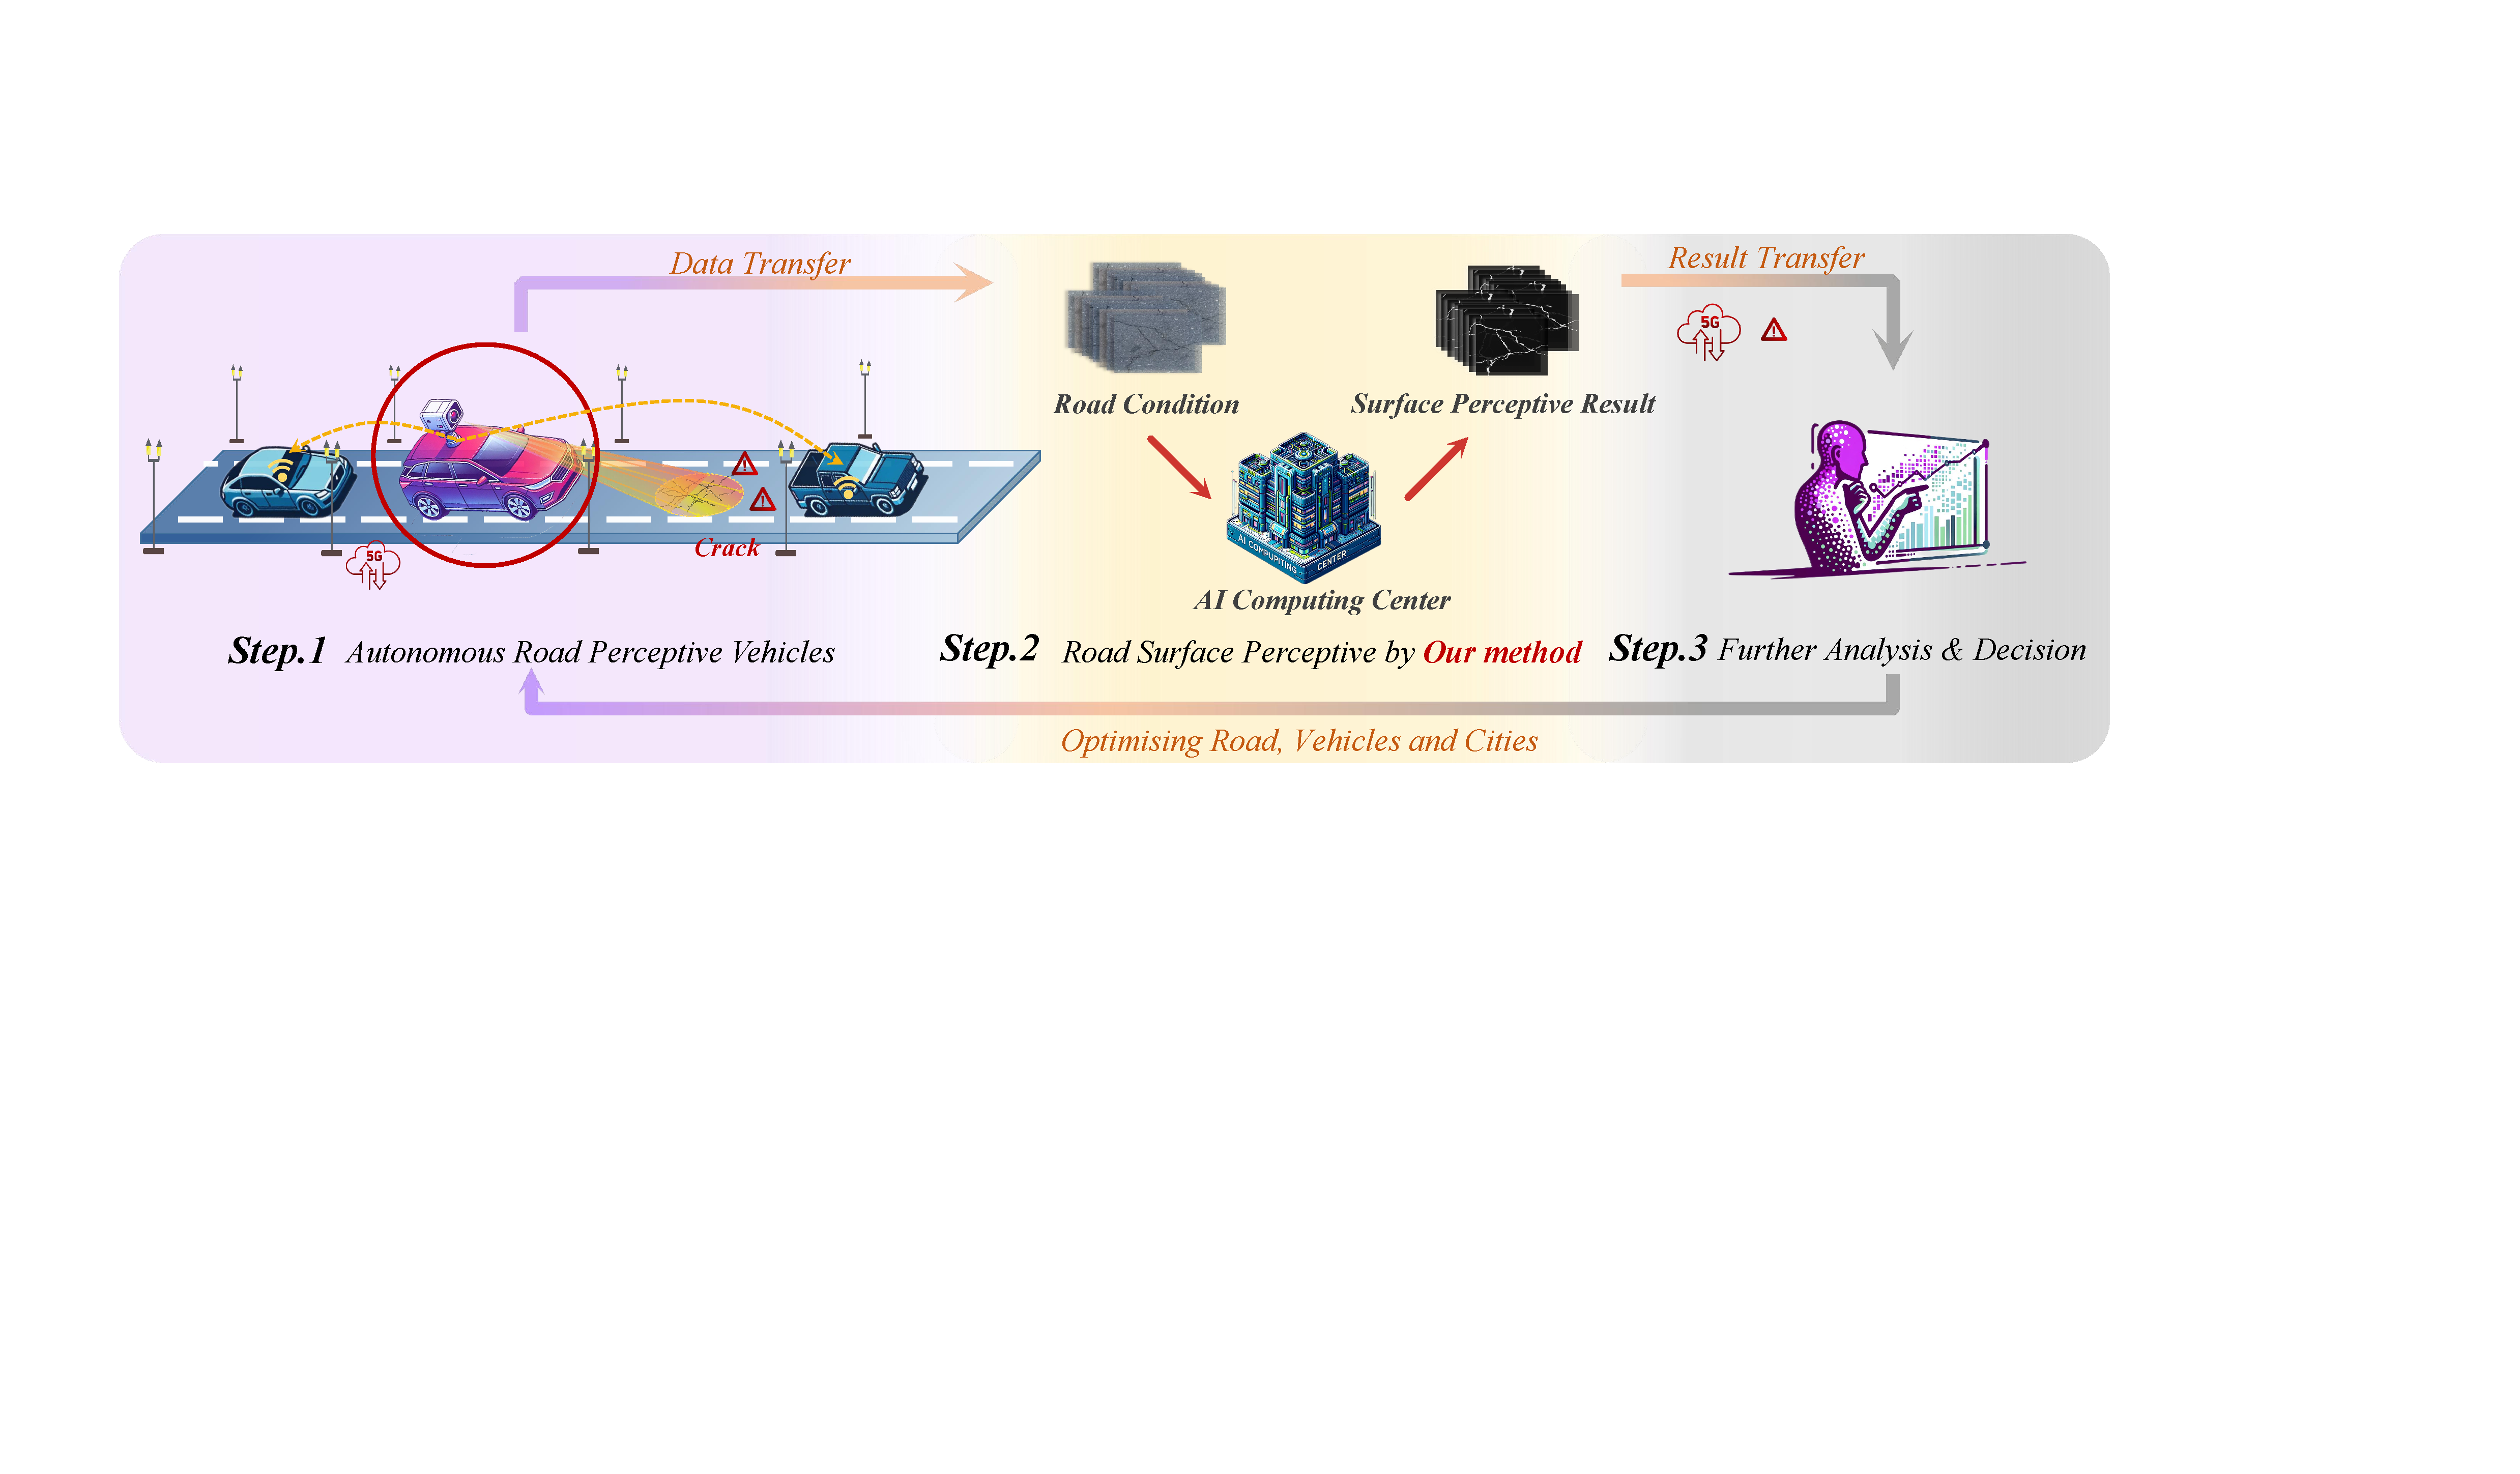
\includegraphics[width=0.95\linewidth]{car0331.pdf}
\caption{The road-perception workflow comprises three steps: capturing road-condition images, detecting cracks with the proposed method, and analyzing and transmitting the results to the vehicles.}
\label{road-perceptive vehicle}
\end{figure*}


Traditional crack detection methods have primarily relied on digital image processing technologies, involving laborious procedures with complex preprocessing and initial crack identification, followed by refinement~\cite{DBLP:conf/icarcv/DinhHL16,DBLP:journals/tits/OliveiraC13}. These techniques, dependent on manually selected features and classical machine learning models, often falter when distinguishing cracks against intricate backgrounds. The advent of deep learning marks a pivotal transition, ushering in a wave of sophisticated algorithms designed for specific types of cracks and conditions. This shift leverages the capabilities of convolutional neural networks (CNNs) to significantly improve road damage detection, utilizing hierarchical feature learning for edge detection~\cite{DBLP:journals/ijon/LiuYLXL19,DBLP:journals/tits/YangZYPML20} and pioneering deep supervision and enhancement techniques for heightened performance. Moreover, multi-scale feature fusion has emerged to effectively marry local and global feature representations, with attention mechanisms fine-tuning feature selection for better discrimination~\cite{DBLP:journals/wicomm/HuHYHL21,DBLP:journals/cacie/QuqaLL23,li2018automatic}.

Despite these advancements, deep learning methods predominantly focus on the RGB domain, searching for textural inconsistencies or `breakthrough points' to pinpoint cracks. Yet, the nuanced characteristics of road surfaces frequently mask these defects, posing significant detection challenges. 


%%%%%%%%%%%%%%%%%%%%%%  R1 - Q1 %%%%%%%%%%%%%%%%%%%%%%



Recently, several studies have introduced frequency-domain cues into image segmentation, such as FsaNet~\cite{DBLP:journals/tip/ZhangPG23}, LGFFM~\cite{11129883TMI}, FMamba~\cite{DBLP:journals/tim/LiuLLWZS25}, and FINet~\cite{DBLP:journals/tcsv/WangZZGY25}. 
Although these methods validate the potential of frequency features, they typically treat frequency information as auxiliary input rather than achieving a deeply coupled frequency-spatial representation. 
For instance, FsaNet focuses only on low-frequency tokens without adaptive fusion with spatial branches, LGFFM employs dual encoders with heavy computation, FMamba emphasizes global consistency while losing fine texture detail, and FINet is restricted to ultrasound imagery. 
These limitations reveal that existing frequency-based networks lack generalization and efficient integration with spatial representations, especially in complex natural scenes.


%%%%%

Addressing this, our study introduces the Frequency-aware network (FANet), a novel architecture that integrates RGB and frequency domain information. This dual-strategy approach aims to overcome the limitations of relying solely on RGB information by enhancing the network's sensitivity to subtle textural features often obscured in the spatial domain. FANet represents a significant leap forward, offering enhanced accuracy in crack detection through a more holistic analysis of road surface characteristics.
FANet commences its detection process with a frequency-guided coarse positioning phase, where the primary aim is to leverage frequency domain features for identifying potential crack locations, known as breakthrough points. Distinguished by a transformer backbone, FANet proficiently extracts different level features from the input. A specialized frequency-aware module (FAM) then distinguishes these features into high- and low-frequency components, which correspond to the texture and contour details of the road surface, respectively. This division allows for a comprehensive representation of the frequency domain, enabling the coarse but accurate localization of road cracks. The process is enhanced by a neighbor interaction mechanism that promotes the integration of frequency-aware features across various levels, facilitating an initial yet refined crack detection.

Transitioning into the detail-preserving fine segmentation phase, FANet refines the previously identified crack locations through a process of prior-guided correction and cross-layer feature fusion. This refinement is achieved with the help of the hybrid fusion module (HFM), which manages the interplay of high-level features across different layers to boost the accuracy of the detection framework. The inclusion of shallow, high-resolution features ensures the meticulous delineation of structural information, leading to the production of the final crack detection output. This dual-phase approach, combining coarse positioning with fine localization, allows FANet to not only detect cracks with high precision but also to discern subtle features that traditional methods might overlook, setting a new standard in the field of road surface monitoring. In Fig. \ref{introdvis}, our proposed framework demonstrates superior performance across all five datasets. 

The core contributions of this paper are listed as follows:

\begin{itemize}
    
    
    \item We propose a two-stage Frequency-Aware Network (FANet) that jointly models spatial and frequency information for robust crack detection. 
    Unlike existing approaches that process frequency cues independently, FANet achieves unified frequency-spatial representation through frequency-guided coarse localization and detail-preserving fine segmentation, 
    significantly enhancing precision and generalization under complex textures and noise.

    \item We design a fully integrated frequency-aware module capable of automatically distinguishing between low- and high-frequency features. This module significantly improves road-crack localization.
    
    \item We introduce a hybrid fusion module that integrates high-level features via prior-guided correction and incorporates shallow features to refine crack details. Results on five datasets demonstrate the effectiveness of FANet.
    
\end{itemize}


\section{Related Work}\label{sec2}


\subsection{Traditional Crack Detection Techniques}
For traditional crack detection, Techniques such as intensity thresholding, morphological analysis, and classical machine learning strategies have been foundational, as evidenced by extensive different researchs~\cite{DBLP:journals/cacie/NishikawaYSF12,DBLP:journals/cacie/YangLYLHY18}. A pioneering approach within this domain is the CrackTree algorithm, delineated in~\cite{DBLP:journals/prl/ZouCLMW12}, which utilizes minimum spanning trees (MSTs) for the automated identification of cracks. Parallel to this, substantial efforts by researchers~\cite{DBLP:journals/ivc/LiZZM11,DBLP:journals/pami/KaulYT12,DBLP:journals/tits/AmhazCIB16} have been devoted to leveraging minimal path techniques for crack region detection. Given the complex, irregular patterns of cracks, numerous strategies have been formulated, emphasizing edge detection and bespoke feature engineering. An innovative methodology reported in~\cite{DBLP:journals/ivc/ZhangLCCHZ17} implements a dual-phase strategy, initiating with Region of Belief (RoB) seed extraction, succeeded by region-growing algorithms to coalesce disjointed regions for enhanced crack identification. Furthermore, the technique introduced in~\cite{DBLP:journals/tits/ShiCQMC16} makes use of random structure forests in crack detection, thereby facilitating a better comprehension of crack structures and diminishing noise artifacts. Nonetheless, these traditional methods, despite their utility in specific contexts, are often challenged by their susceptibility to noise and a heavy reliance on manual feature extraction, limiting their effectiveness in more intricate scenarios.



\begin{figure*}[!hbpt]
\centering
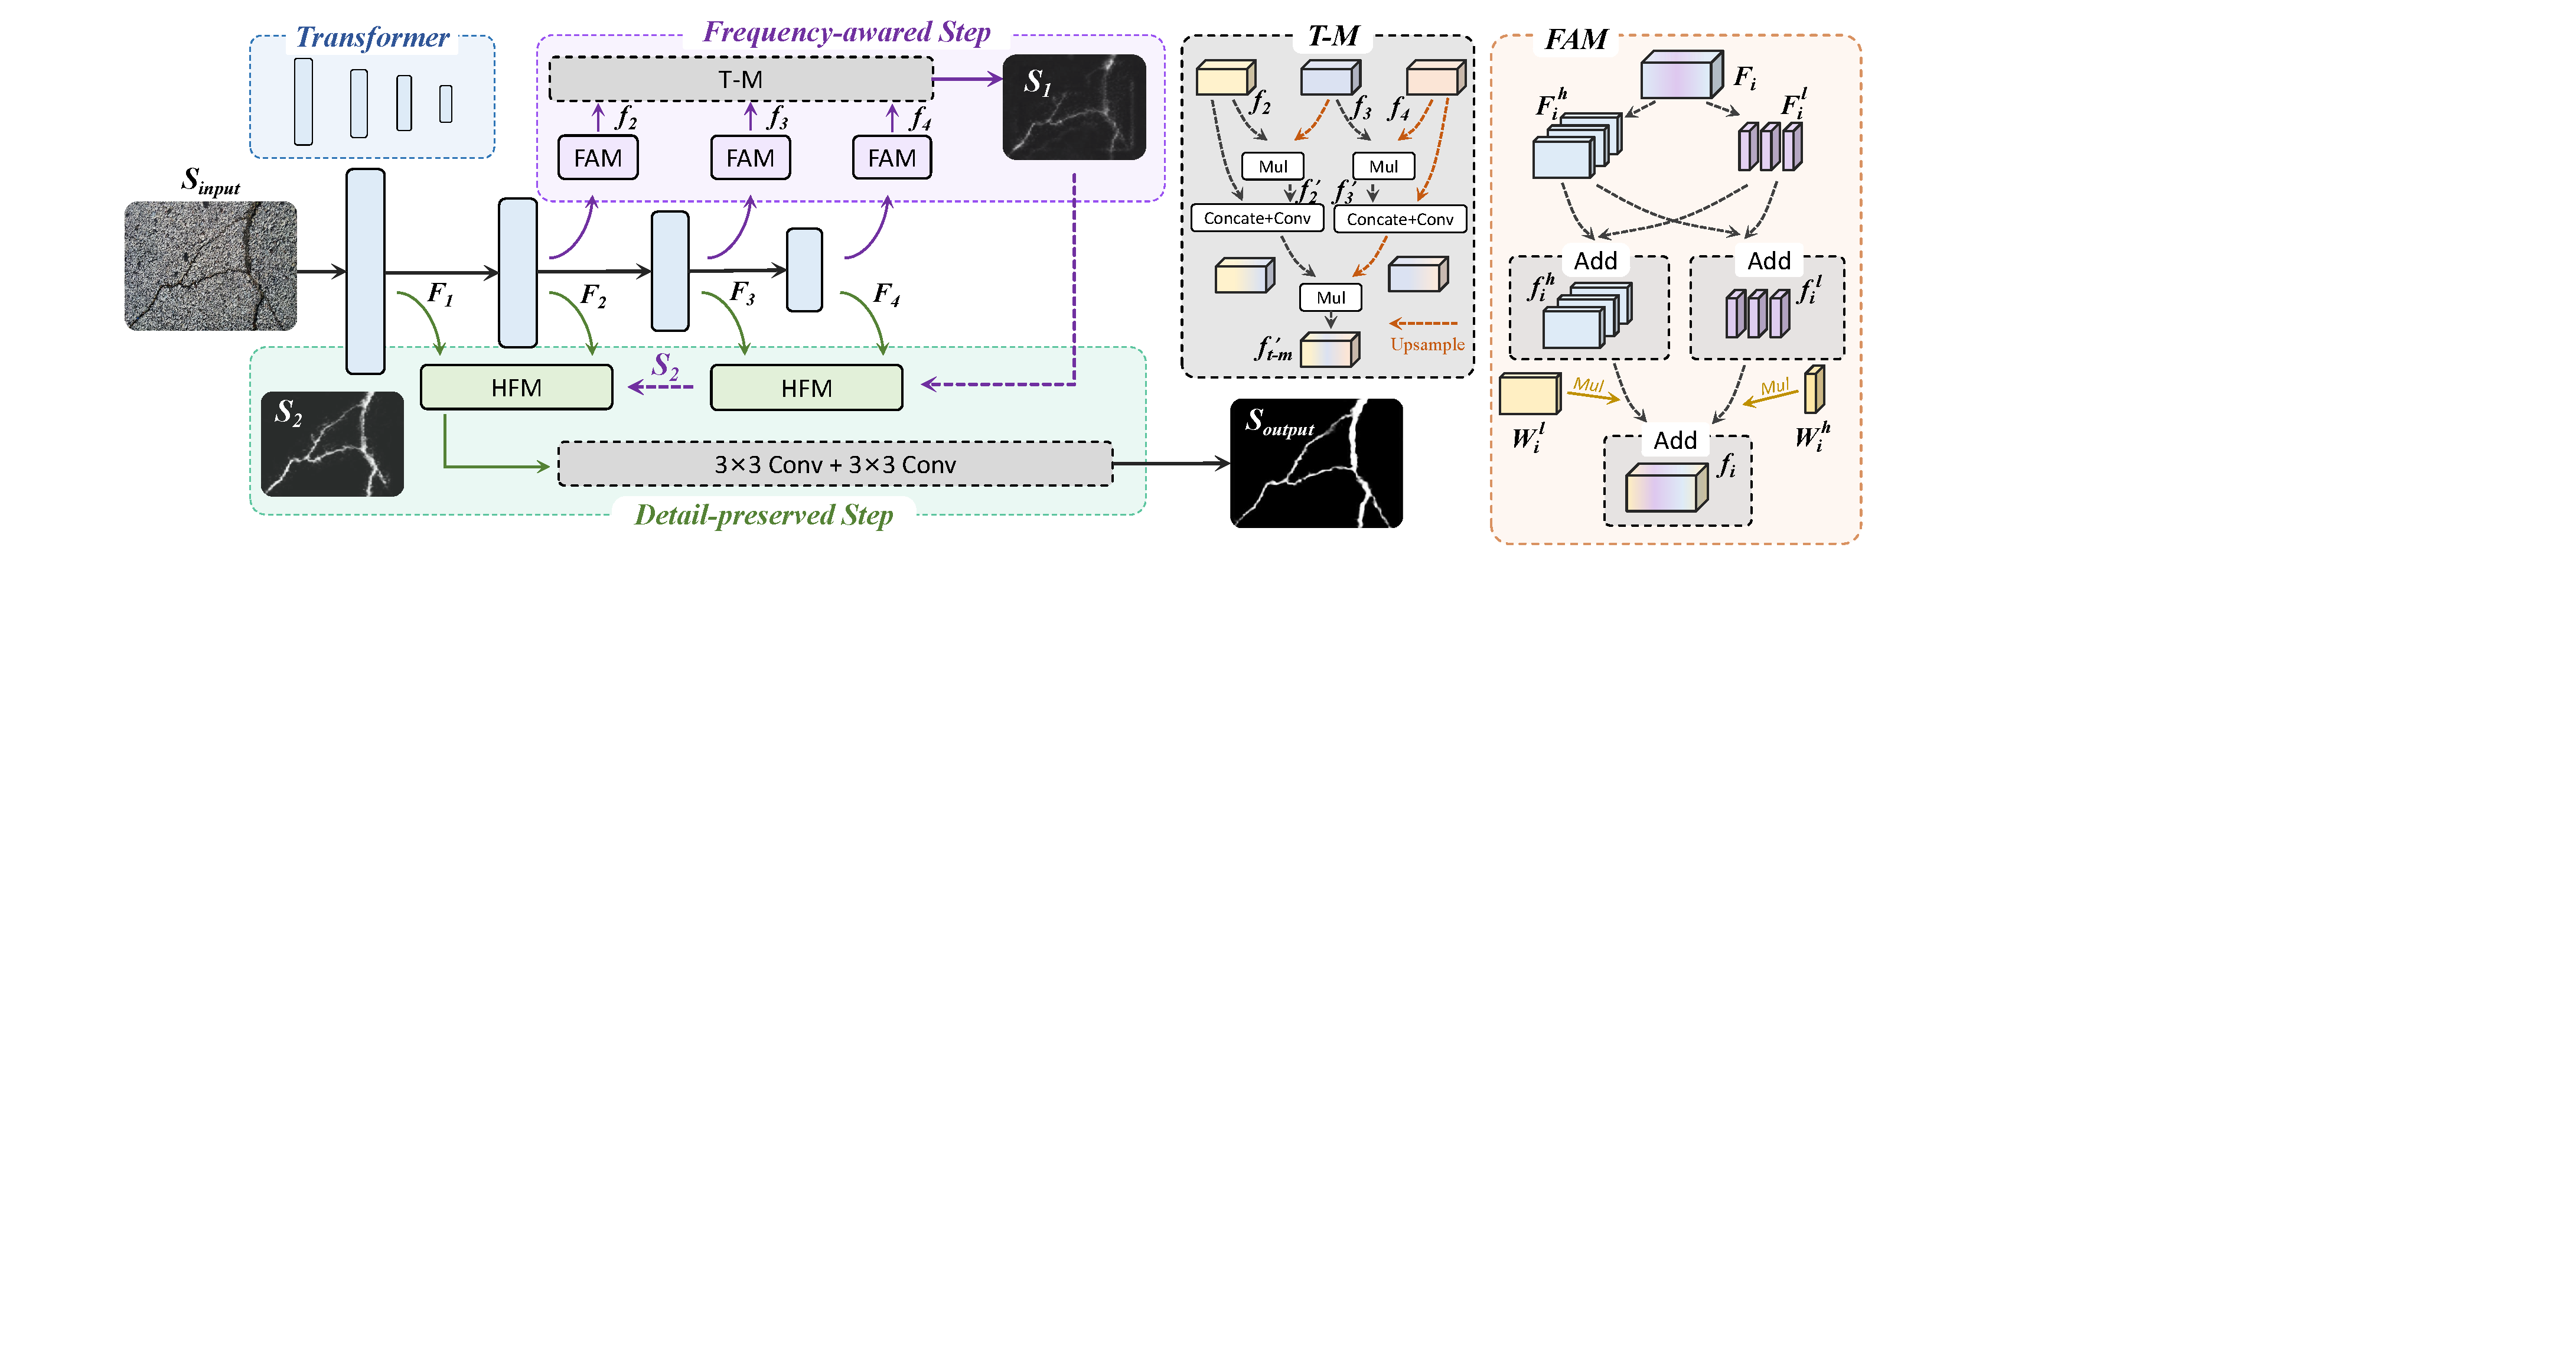
\includegraphics[width=\linewidth]{framework1019.pdf}
\caption{Overall architecture of the proposed Frequency-Aware Network (FANet). 
The solid arrows denote feature flow between modules, while dashed lines represent skip connections used for cross-layer feature fusion. 
Each block (FAM, HFM, and Transformer-based backbone) corresponds to a specific processing stage described in Sections~\ref{overview} to~\ref{sec:Detail-preserving-Fine-Localization}.}
\label{Framework}
\vspace{-0.5cm}
\end{figure*}




\subsection{Advancements in Crack Detection via Deep Learning}

The realm of crack detection has witnessed a transformative shift with the advent of deep learning technologies, heralding a new epoch of innovation and efficiency. This period is characterized by breakthroughs in deep learning that have revolutionized not only detection but also classification and segmentation within various fields~\cite{Hu2025,DBLP:journals/pami/ChenLLSWZ21,KUANG2024100146,PENG2025100170}. Central to these advancements is the ability of deep learning models to autonomously discern and abstract pivotal, high-level features via an end-to-end learning process. 
This capability has driven rapid progress in applying deep learning to crack detection tasks~\cite{DBLP:journals/cacie/RodriguezLozanoGPO23, DBLP:journals/cacie/ZhouZG23}.



For example, an innovative hierarchical segmentation network that integrates FCNs with Conditional Random Fields (CRFs) and Guided Filtering (GF) is introduced in~\cite{DBLP:journals/ijon/LiuYLXL19}, aiming to exploit multi-layer features for meticulous refinement. Following this, encoder-decoder based FCNs have been developed, tailored to discriminate between crack and non-crack pixels with high precision~\cite{DBLP:journals/LD}. The DeepCrackT model, as proposed in~\cite{DBLP:journals/tip/ZouZLQWW19}, enhances the encoder-decoder framework through a novel pairwise fusion technique of crack features at corresponding scales, significantly boosting detection capabilities. In pursuit of computational efficiency, the introduction of a lightweight crack detection network marks a significant milestone, incorporating split-exchange convolution and multi-scale feature fusion to streamline network operations and expedite detection processes~\cite{DBLP:journals/tiv/ZhouQJ23}.

However, relying solely on RGB information presents a significant limitation~\cite{ZHUANG2025100194}, as the spatial domain represented by RGB channels provides a direct yet occasionally superficial perspective of image content, potentially overlooking subtle features more discernible in the frequency domain. Recognizing this shortfall, our work introduces an innovative approach that incorporates frequency domain information into the crack detection process. By leveraging the frequency domain, we aim to reveal a wider spectrum of features, leading to more accurate and robust crack detection.


In addition to conventional RGB-based frameworks, several recent studies have explored incorporating frequency-domain cues into image segmentation. 
For instance, FsaNet~\cite{DBLP:journals/tip/ZhangPG23} applies a discrete cosine transform (DCT) to enhance low-frequency representations, 
yet it lacks adaptive interaction between frequency and spatial branches, limiting its generalization to texture-rich or noisy environments. 
LGFFM~\cite{11129883TMI} introduces a dual-encoder structure combining CNN and Transformer backbones along with a Frequency Domain Mapping Module, 
which improves global perception but incurs high computational complexity and training instability. 
FMamba~\cite{DBLP:journals/tim/LiuLLWZS25} embeds frequency enhancement into a lightweight Vision Mamba backbone, 
providing efficient feature extraction but prioritizing sequential consistency rather than fine-grained local texture cues. 
FINet~\cite{DBLP:journals/tcsv/WangZZGY25} proposes a frequency-aware self-attention mechanism for ultrasound image segmentation, 
but it is task-specific and not easily generalizable to natural road scenes.




These methods collectively demonstrate the potential of frequency features in segmentation, 
yet they generally treat frequency cues as auxiliary enhancements rather than deeply integrating them with spatial representations. 
\textbf{In contrast, our proposed FANet establishes a unified two-stage frequency-spatial synergy, 
where the frequency-guided coarse localization phase captures global structure and the detail-preserving fine segmentation phase refines local details.} 
This design enables dynamic modulation between spectral and spatial features, achieving superior robustness, precision, and adaptability under complex road textures and illumination variations.

\textcolor{red}{More recent studies from the past two years further advance both crack detection and frequency-aware representation learning. On the crack-detection side, UP-CrackNet~\cite{TITS24_UPCrackNet} formulates road crack detection as unsupervised adversarial image restoration to remove the dependence on pixel-wise annotations; SCSegamba~\cite{CVPR25_SCSegamba} designs a lightweight structure-aware vision Mamba that captures crack morphology and texture with minimal computational cost; and an ultra-lightweight Mamba network with frequency-domain feature extraction has been developed for pavement tiny-crack segmentation~\cite{ESWA25_MambaFreqCrack}. On the frequency-modeling side, FreqFusion~\cite{TPAMI24_FreqFusion} rectifies feature fusion for dense prediction with adaptive low-/high-pass filters, and FSEL~\cite{ECCV24_FSEL} entangles frequency and spatial representations for camouflaged object detection. Closely related inspection and segmentation problems have also been actively studied in IEEE Transactions on Cybernetics, including zero-shot industrial anomaly detection with hybrid vision-language prompts~\cite{TCYB25_AnomalyVLM} and contrastive transformer-based segmentation of subtle structures~\cite{TCYB24_CTNet}. These advances confirm the growing interest in spectral cues and efficient architectures; however, they either address generic dense prediction or treat frequency information as an auxiliary enhancement, leaving a deeply coupled frequency-spatial representation dedicated to road crack detection, the very focus of FANet, largely unexplored.}





\section{Proposed Method}
\subsection{Overview} \label{overview}
Our objective is to harness and integrate the unique benefits of both the RGB and frequency domains, aiming to boost the discriminative capabilities for detecting road cracks via intelligent road-perceptive vehicles. In pursuit of this, we present the FANet, a novel architecture tailor-made for crack detection, as depicted in Fig.~\ref{Framework}. FANet is architected around three core components: the Transformer-based feature extraction, the frequency-guided coarse crack localization step, and the detail-preserving fine crack segmentation step. Given an input image $S \in \mathbb{R}^{H \times W \times 3}$, FANet begins with the feature extraction with the Pyramid Vision Transformer (PVT)~\cite{DBLP:journals/cvm/WangXLFSLLLS22} as its feature extractor. This feature extractor generates multi-level feature maps $F_i$, $i \in \{1,2,3,4\}$, each catering to different facets of the detection challenge. The first-level feature map $F_1$, captures intricate details of the road surface essential for spotting minor cracks, whereas the subsequent levels ($F_2, F_3, F_4$) encapsulate progressively higher-level semantic information, pivotal for robust crack localization. In the frequency-guided coarse crack localization phase, our proposed novel frequency-aware module (FAM) extracts frequency domain features from the high-level features ($F_2, F_3, F_4$), which are then synergized using a {tri-merge (T-M) decoder}. This process yields a preliminary crack map $S_1$. 

After the coarse step, the detail-preserving fine crack segmentation step refines the initial map by using $S_1$ to steer the embedding of high-level features into a hybrid fusion module (HFM). This module facilitates layer-wise, prior-guided adjustments and fusion, significantly enhancing segmentation accuracy. After this step, the final ouput crack map is $S_{\text{output}}$.

\begin{figure}
\centering
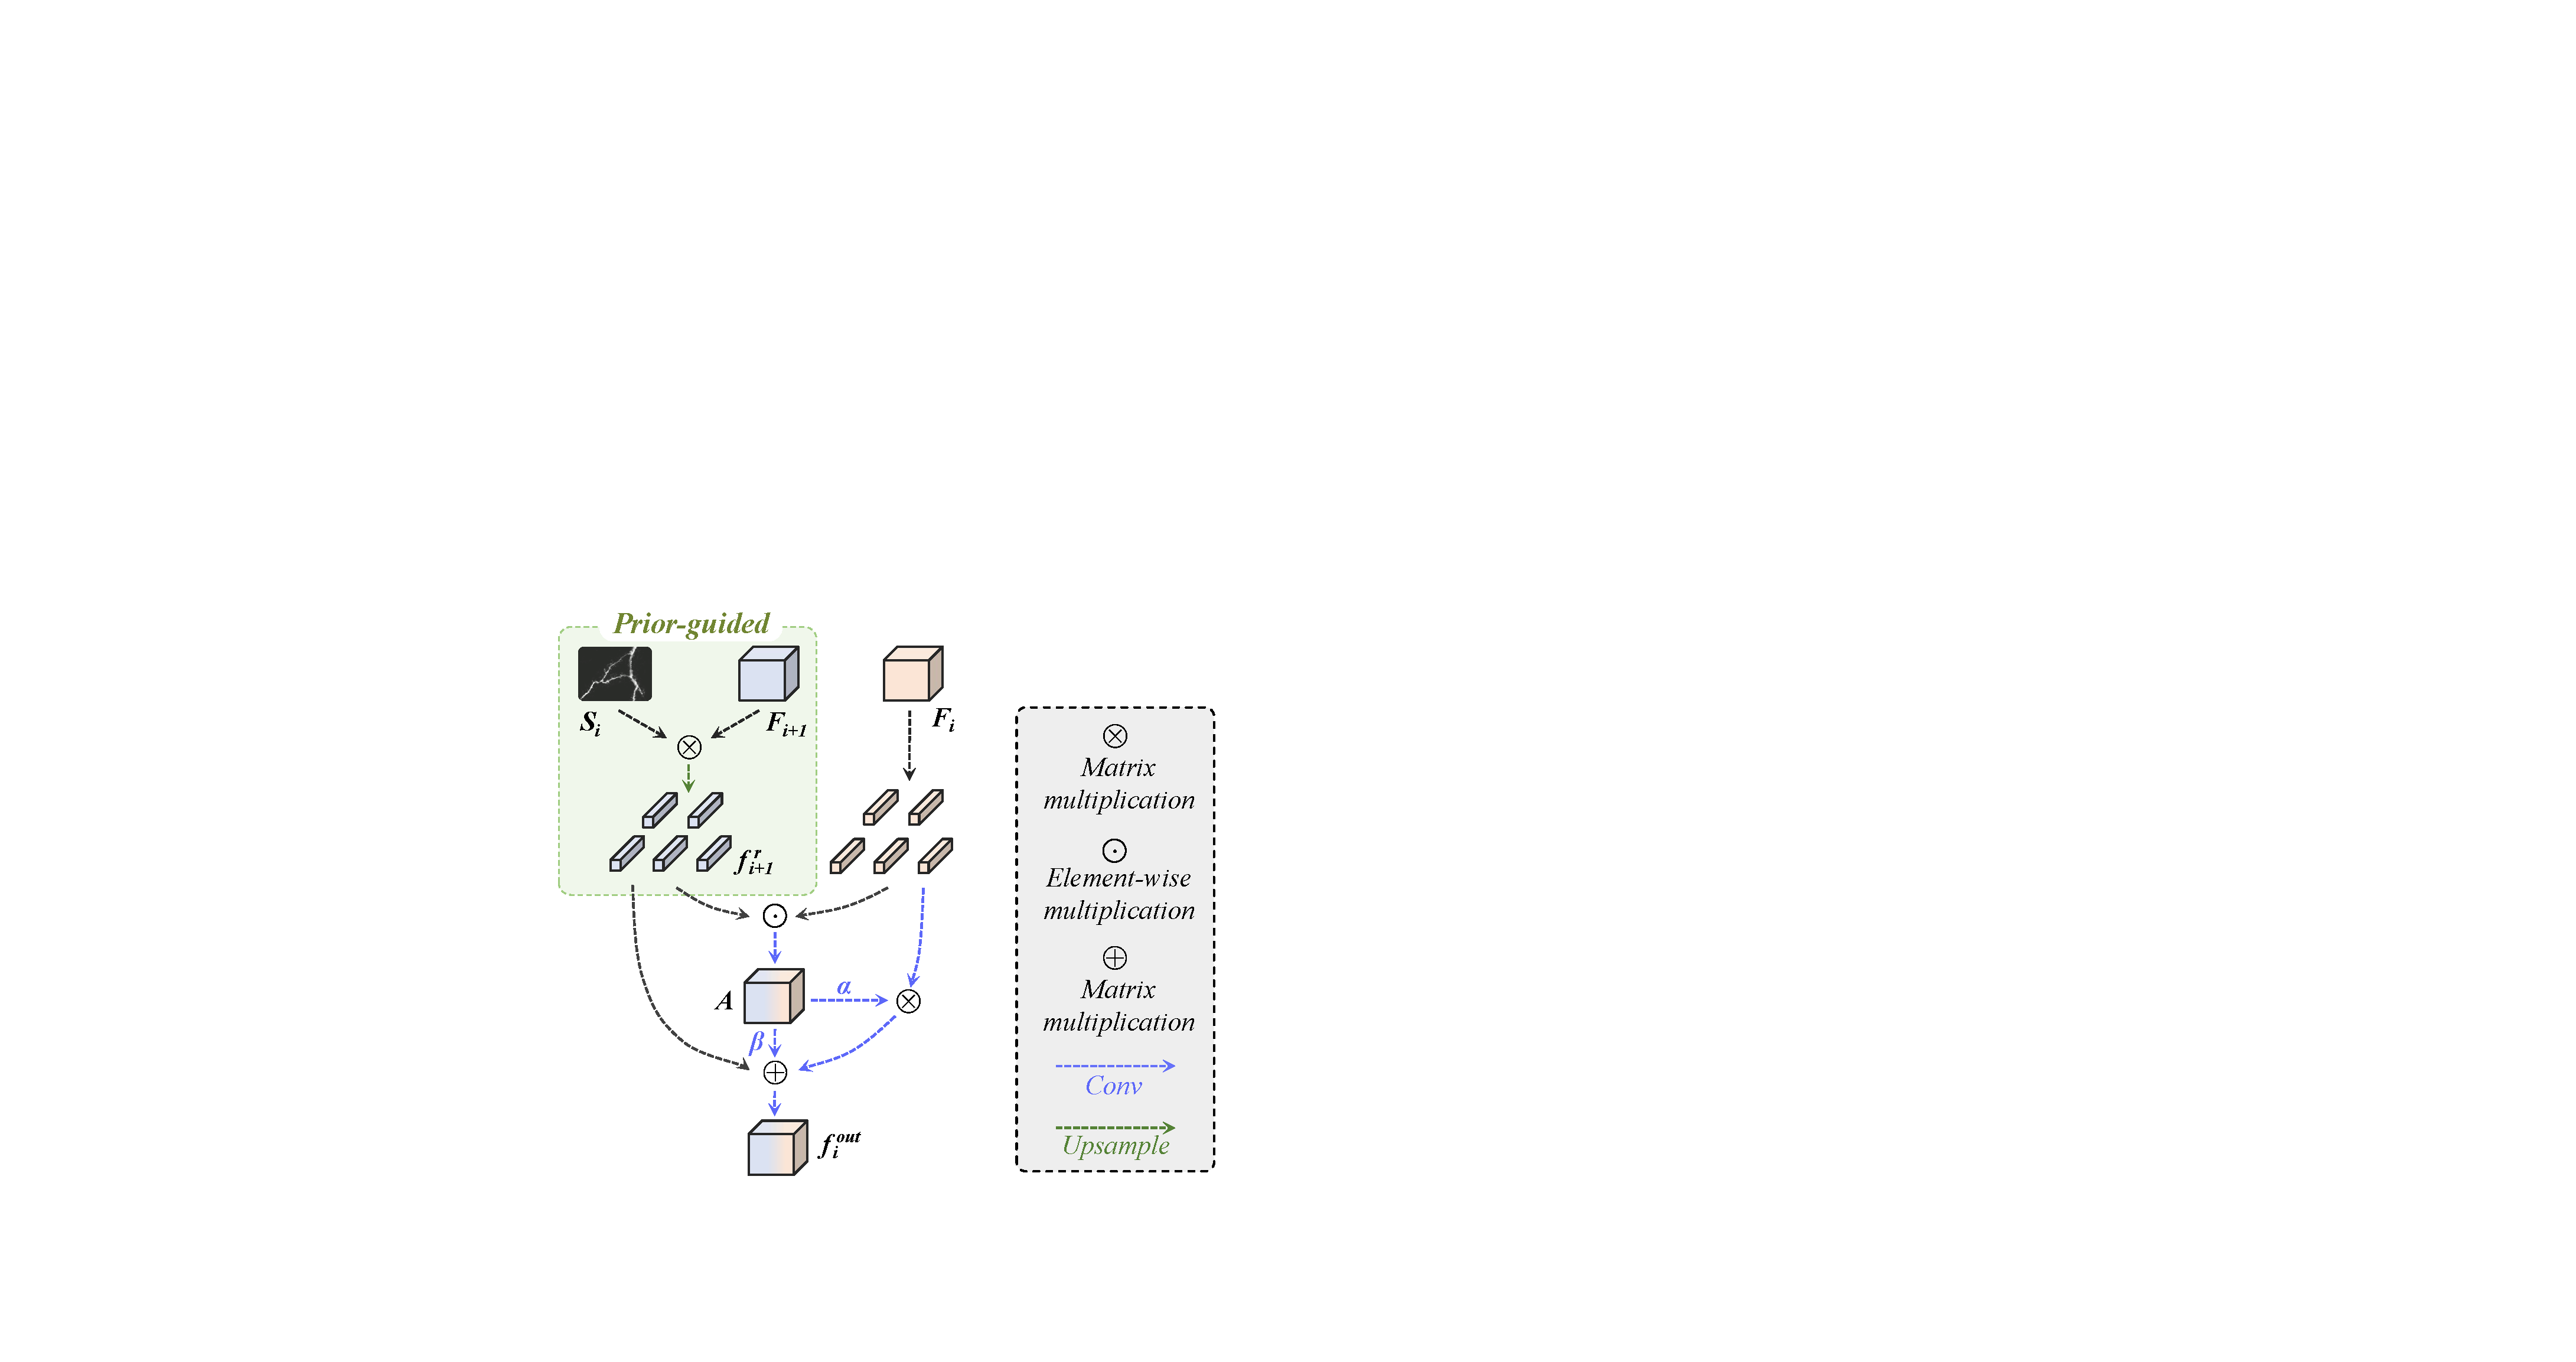
\includegraphics[width=0.75\linewidth]{HFM_0617.pdf}
\caption{{The architecture of our proposed hybrid fusion module (HFM).}}
\label{HFM}
\vspace{-0.5cm}
\end{figure}

\subsection{{Frequency-guided Crack Localization}} \label{sec:Frequency-guided-Coarse-Positioning}
\textcolor{red}{\textbf{Design intuition of FAM.} Road cracks appear as sparse and sharp intensity discontinuities embedded in slowly varying pavement context. In the feature space, the former concentrates in the high-frequency band, whereas the latter dominates the low-frequency band. The FAM is therefore designed to (i) decompose each backbone feature into high- and low-frequency components, (ii) let the two components exchange complementary information so that edge responses acquire contextual support and contour responses are cleansed of texture noise, and (iii) adaptively re-weight and merge the two bands with learnable weights. The output is a frequency-balanced feature in which crack evidence is amplified relative to background texture. The remainder of this subsection formalizes these three steps.}

Unlike an offline DCT preprocessing stage, Octave Convolution~\cite{DBLP:conf/iccv/Chen0XYKRYF19} factorizes a feature map $F_i$ into high- and low-frequency components $\{F_i^h,F_i^l\}$ within the network. The high-frequency branch captures rapidly varying textures and edges, whereas the lower-resolution low-frequency branch models smoothly varying contextual structures. As shown in Fig.~\ref{Framework}, FAM exchanges information between these branches as follows:

\begin{equation}
f^{h}_{i} = Conv(F^{h}_{i}) + \text{Upsample}(Conv(F^{l}_{i}), 2),
\end{equation}

\begin{equation}
f^{l}_{i} = Conv(F^{l}_{i}) + Conv(\text{Pool}(F^{h}_{i}, 2)),
\end{equation}
where $\text{Pool}(X, k)$ represents average pooling with a $k \times k$ kernel, and $\text{Upsample}(X, s)$ signifies upsampling by a scale factor of $s$ through nearest neighbor interpolation. 

The exchanged components are resized to a common resolution and combined using learnable weights:
\begin{equation}
f_i = \{ \text{Resize}(f^{h}_{i}) \odot W^{h}_{i} \} \oplus  \{ \text{Resize}(f^{l}_{i})  \odot W^{l}_{i}  
 \},
\end{equation}
where $\text{Resize}$ adjusts the features to a common spatial resolution, $W^{h}_{i}$ and $W^{l}_{i}$ are learnable weights, $\oplus$ denotes element-wise addition, and $\odot$ denotes element-wise multiplication.


\textcolor{red}{\textbf{Design intuition of T-M.} The T-M decoder aggregates the frequency-aware features of the three deepest levels: deeper features indicate \emph{where} a crack is likely to exist, while shallower ones describe its shape more precisely. Multiplying adjacent levels retains only the responses that are confirmed by both, yielding a clean coarse localization map $S_1$.}

The T-M decoder implements this adjacent-level interaction as follows:

\begin{equation}
\begin{split}
    f'_3 &= Conv^ {\uparrow }(f_4)   \odot f_3, \\
    f'_2 &= Conv^ {\uparrow }(f_3)   \odot f_2, \\
    g_2 &= Conv(\text{Cat}(f_2,f'_2)), \\
    g_3 &= Conv(\text{Cat}(f_3,f'_3)), \\
    f'_{t-m} &= g_2 \odot \text{Upsample}(g_3,2).
\end{split}
\end{equation}

Here, $Conv^{\uparrow}$ represents upsampling followed by a $3 \times 3$ convolution, and $\text{Cat}(A,B)$ denotes feature concatenation. The two concatenated features are convolved, $g_3$ is upsampled to the resolution of $g_2$, and their element-wise product $f'_{t-m}$ is decoded into the coarse crack map $S_1$.



\subsection{{Detail-preserving Crack Segmentation}} \label{sec:Detail-preserving-Fine-Localization}

\textcolor{red}{\textbf{Design intuition of HFM.} The HFM addresses two questions during refinement. The first is \emph{where to refine}: at refinement stage $i$, the current guidance map $S_i$ acts as a spatial prior that amplifies crack-relevant regions of the deeper feature. The second is \emph{what to keep}: a channel-level association between adjacent layers determines which high-resolution details are consistent with this prior and should be preserved. These operations refine accuracy with a moderate throughput cost, as quantified in Table~\ref{abla}. The following formulation details the two steps.}

As shown in Figs.~\ref{Framework} and~\ref{HFM}, each HFM takes adjacent 64-channel features $F_i$ and $F_{i+1}$ together with the current guidance map $S_i$. The first HFM uses the coarse map $S_1$; its intermediate prediction provides $S_2$ to the next HFM. At stage $i$, prior-guided refinement is computed as

\begin{equation}
f^r_{i+1} = \text{Upsample}(S_i \otimes F_{i+1}).
\end{equation}

The prior-weighted deeper feature is then associated with the adjacent higher-resolution feature through a $3 \times 3$ convolution:

\begin{equation}
A = Conv(F_{i} \odot (f^r_{i+1})).
\end{equation}

Two weight maps, $\alpha$ and $\beta$, are derived from $A$ using separate $3 \times 3$ convolutions and used to fuse the adjacent features:

\begin{equation}
f^{out}_{i} = f^r_{i+1} + Conv(F_{i}) \otimes \alpha + \beta.
\end{equation}

Here, $\otimes$ denotes matrix multiplication and $\odot$ denotes element-wise multiplication, consistent with the operators in Fig.~\ref{HFM}.

After the two refinement stages, two $3 \times 3$ convolutions generate the final prediction $S_{\text{output}}$.

\textbf{Loss Function.} In alignment with standard practices, we train the FANet through binary cross-entropy loss:
\begin{equation}
L = BCE(S_{\text{output}},\mathcal{G}^T),
\end{equation}
where $\mathcal{G}^T$ is the ground-truth.


%%%%%%%%%%%%%%%%%%%%%%%%%%%%%%%%%%%%%%%%%%%


\begin{figure*}[!t]
\centering
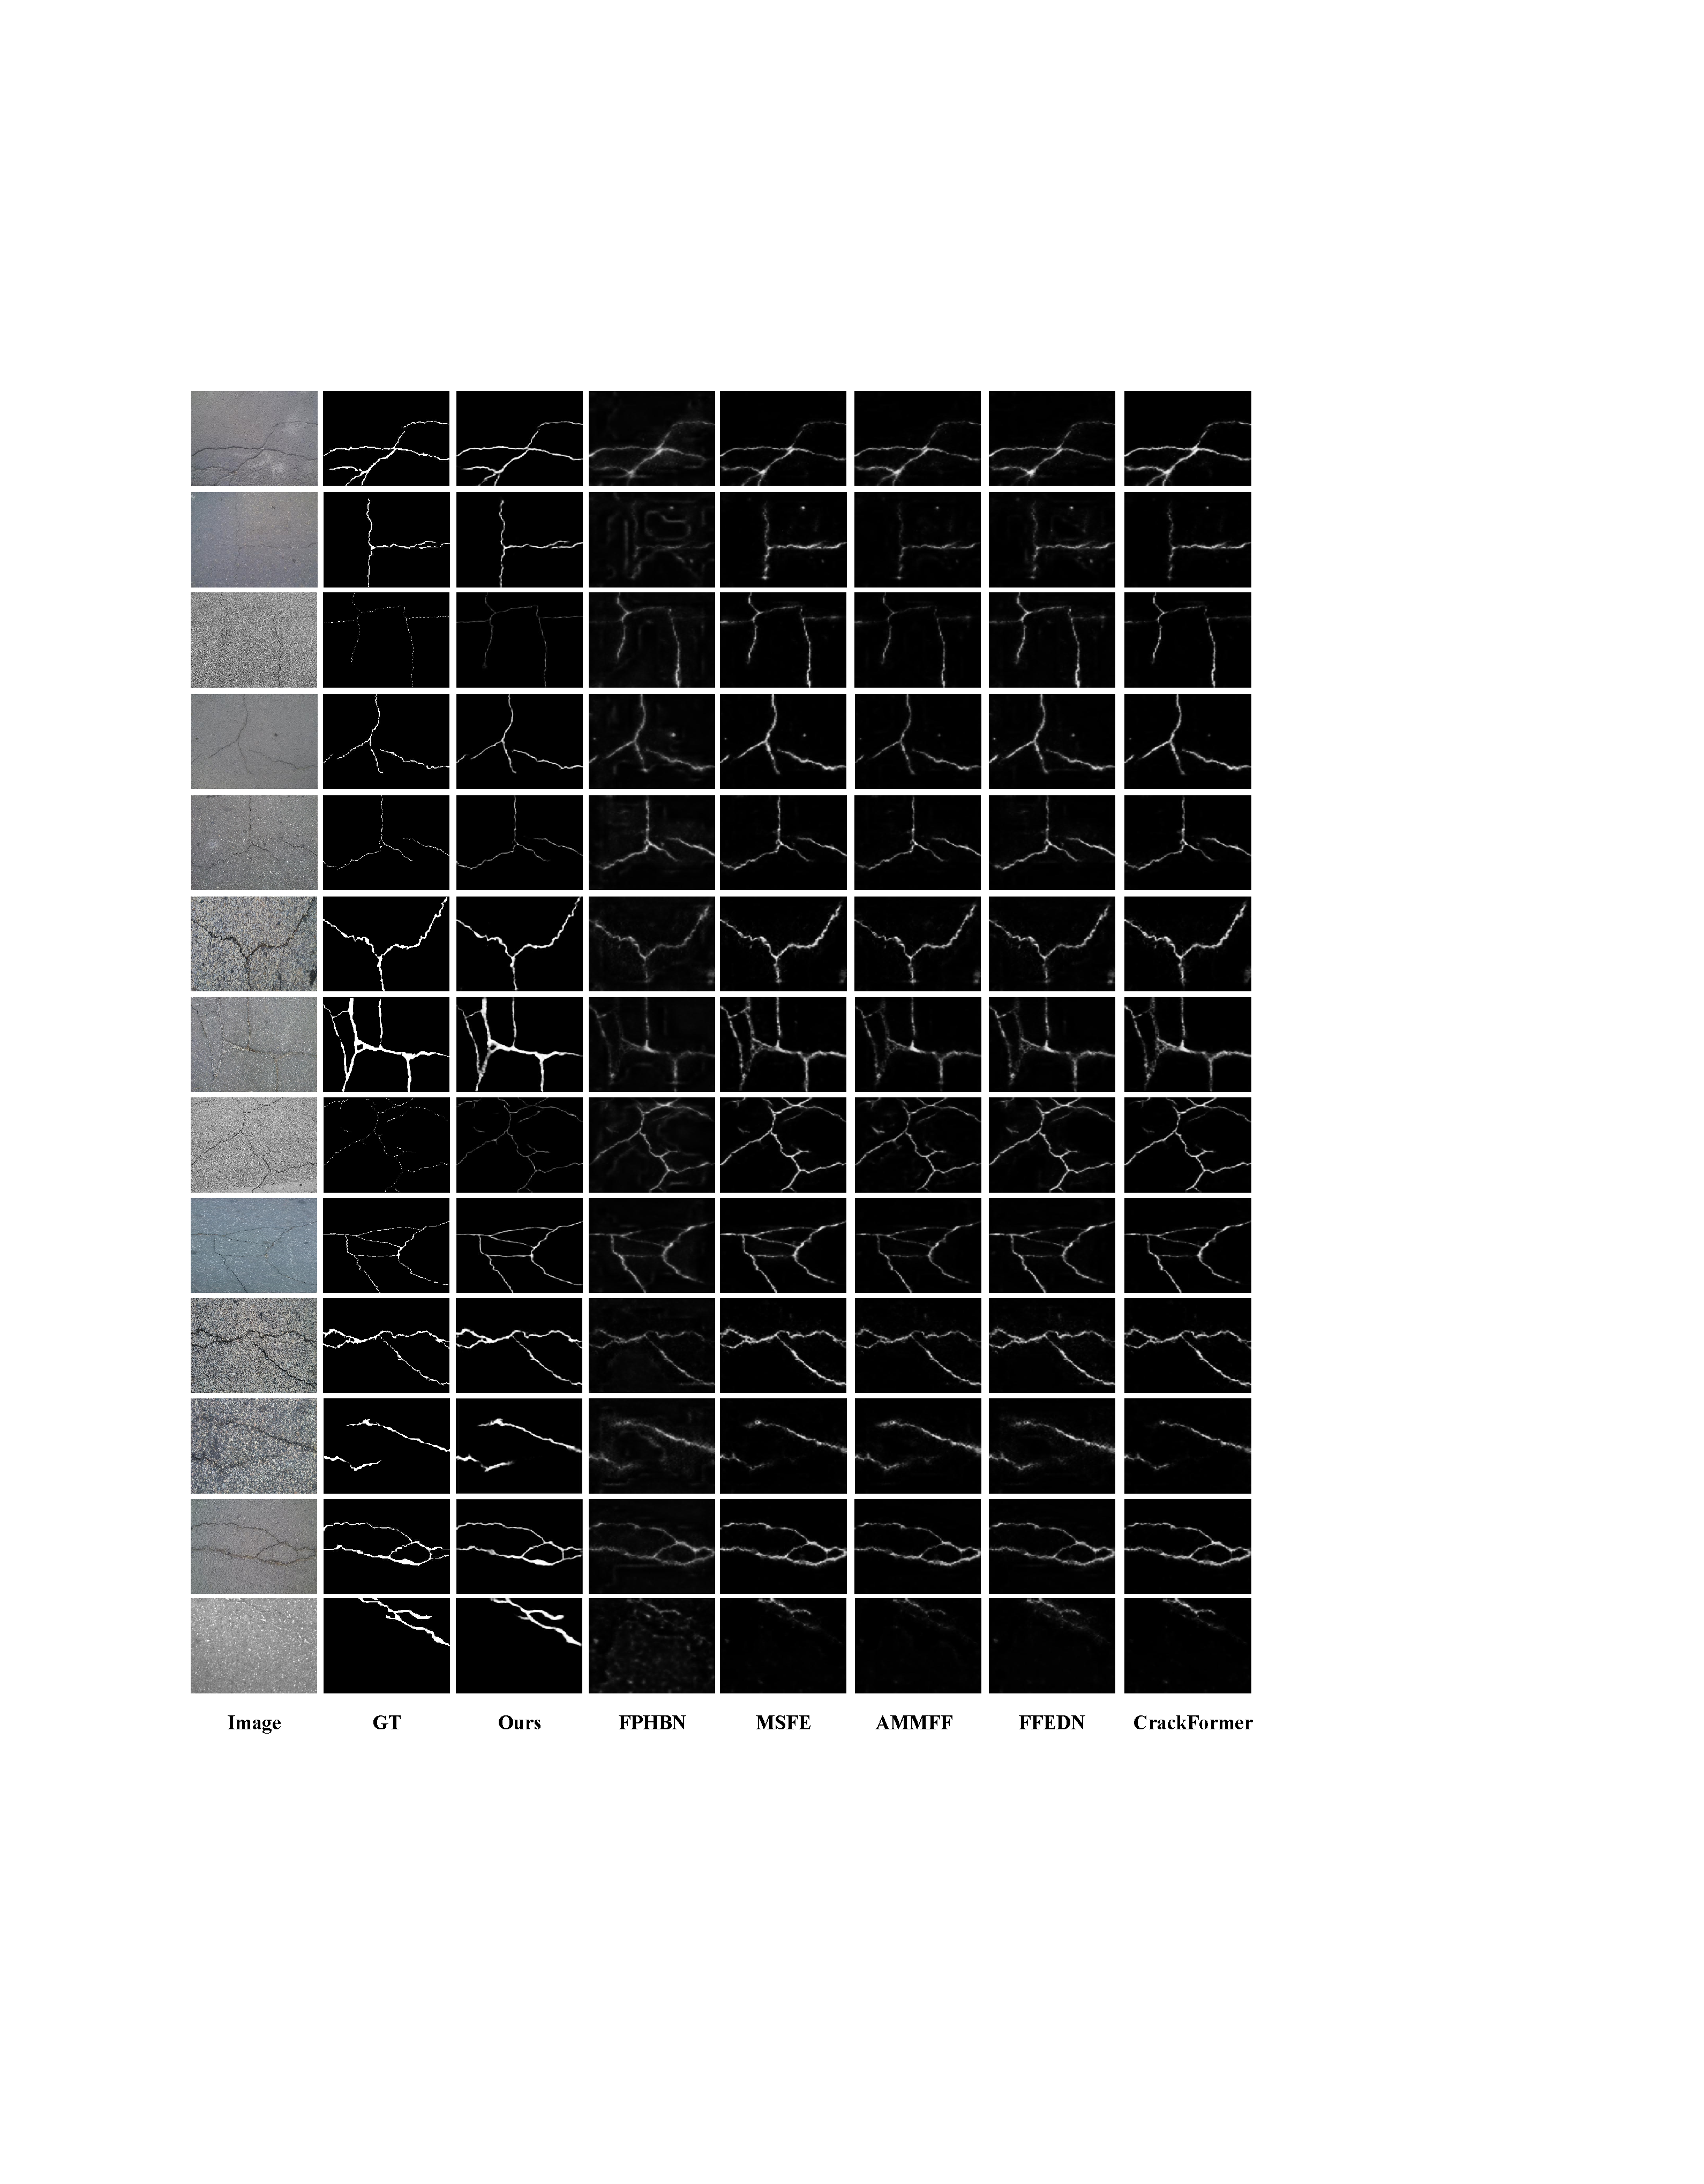
\includegraphics[width=0.9\linewidth]{com0322.pdf}
\caption{Comparison between our FANet and other SOTA methods. It can be clearly observed that FANet achieves impressive performance in all these cases. Best viewed by zooming in.}
\label{QualitativeResults}
\end{figure*}


\section{Experiments}
\subsection{Implementation Details}
FANet uses an ImageNet-pretrained PVT backbone and is implemented in PyTorch. We use the Adam optimizer with an initial learning rate and weight decay of $1 \times 10^{-4}$. Input images are resized to $512 \times 512$, and the model is trained for 100 epochs on an NVIDIA RTX 3090 Ti GPU with a mini-batch size of 4. Random flipping and cropping are used for data augmentation.





\subsection{Datasets for Evaluation}
Our model's efficacy is rigorously assessed using five widely recognized datasets, each offering unique challenges that simulate the complexities of crack detection scenarios.

\textbf{Crack500}~\cite{DBLP:journals/tits/YangZYPML20}: A comprehensive dataset tailored for crack detection, Crack500 consists of 500 images, partitioned into 250 for training, 50 for validation, and 200 for testing. It encompasses a diverse array of crack conditions, including but not limited to occlusions, variable contrast, shadow effects, and ambient noise, accurately mirroring the intricate nature of real-life crack detection challenges.

\textbf{GAPs384}~\cite{DBLP:conf/ijcnn/EisenbachSSADSE17,DBLP:journals/tits/YangZYPML20}: GAPs384 is derived from 384 annotated road images selected from the GAPs dataset. After cropping, the benchmark used in our experiments contains 509 image--mask pairs with resolutions of either $640 \times 540$ or $440 \times 540$.

\textbf{CFD}~\cite{DBLP:journals/tits/ShiCQMC16}: Specializing in cracks on concrete surfaces, the CFD dataset includes 118 images, each sized at $480 \times 320$. The dataset is characterized by its portrayal of common real-world disturbances such as uneven lighting, shadows, obstructions, and moisture accumulation, thus providing a robust platform for evaluating crack detection algorithms.

\textbf{Cracktree200}~\cite{DBLP:journals/prl/ZouCLMW12}: Comprising 206 images of pavement cracks at a resolution of $800 \times 600$, Cracktree200 emphasizes the detection of slender crack formations. The dataset is notable for its representation of fine cracks amidst complex backgrounds, including tree shadows, ambiguous road markings, and the intersection of cracks with such road features.



\textbf{AEL}~\cite{DBLP:journals/tits/AmhazCIB16}: The AEL dataset amalgamates three subsets: Aigle-RN, ESAR, and LCMS. Aigle-RN includes 38 pixel-annotated images for the assessment of French pavements, whereas ESAR and LCMS offer 15 and 5 images, respectively, without specified lighting conditions, further diversifying the dataset's utility in crack detection research.



%%%%%%%%%%%%%%%%%%%%




%%%%%%%%%%%%%%%%%%%%%%%%%%%%%%%%%%%%%%%%%%%


%%%%%%%%%%%%%%%%%%%%%%%%%



%%%%%%%%%%%%%%%%%%%%%%%%%%%%   3  %%%%%%%%%%%%%%%%%%%%%%%%%%%%%%



%%%%%%%%%%%%%%%%%%%%



\begin{table*}[!t]
\centering
\caption{Comparison with other methods using F1, AIU, and AP on five datasets, together with FPS measured on the same hardware. Higher values are better. Values in \textcolor{red}{red} and \textcolor{green!50!black}{green} indicate the best and second-best results for each metric, respectively; tied second-best values are both marked.}
\scalebox{0.7}{
\begin{tabular}{@{}cc|cccccccccccccccccc@{}}
\toprule
\multicolumn{2}{c|}{}                                           & \multicolumn{18}{c}{Method}                                                                                                                                                                                                                                                                                                                                                                                                             \\ \cmidrule(l){3-20} 
\multicolumn{2}{c|}{\multirow{-2}{*}{Metric}}                   & \textit{BASNet} & \textit{FPHBN} & \textit{SegNet} & \textit{FCN}                & \textit{D-Crack} & \textit{UHDN} & \textit{D-CrackM} & \textit{UNet} & \textit{FFEDN}               & \textit{CrackF-r} & \textit{MSFE}                & \textit{AMMFF}               & \textit{HFF}                 & \textit{CarNet}              & \textit{FsaNet}              & \textit{LGFFM} & \textit{FMamba} & \textit{Ours}                \\ \midrule
\multicolumn{2}{c|}{\textit{FPS}}                               & 7.9   & 9.3           & 8.6            & 8.8 & 6.9             & 8.6          & 11.4              & 9.3          & 9.4                         & 10.5              & 11.9                         & 10.5                         & 8.8                        & {\color[HTML]{548235}22.2 }                        & {\color[HTML]{FF0000}25.6 }                        & 16.2           & 11.3            &  10.2  \\ \midrule
\multicolumn{1}{c|}{}                            & \textit{AIU} & 0.508           & 0.492          & 0.500           & 0.383                       & 0.505            & 0.471         & 0.440             & 0.443         & 0.492                        & 0.498             & 0.495                        & 0.507                        & 0.494                        & 0.503                        & {\color[HTML]{00B050} 0.535} & 0.527          & 0.522           & {\color[HTML]{FF0000} 0.563} \\
\multicolumn{1}{c|}{}                            & \textit{AP}  & 0.510           & 0.498          & 0.510           & 0.385                       & 0.510            & 0.473         & 0.444             & 0.449         & 0.501                        & 0.505             & 0.496                        & 0.515                        & 0.501                        & 0.511                        & {\color[HTML]{00B050} 0.545} & 0.538          & 0.532           & {\color[HTML]{FF0000} 0.572} \\
\multicolumn{1}{c|}{\multirow{-3}{*}{Crack500}}  & \textit{F1}  & 0.689           & 0.681          & 0.649           & 0.529                       & 0.678            & 0.684         & 0.659             & 0.678         & 0.624                        & 0.640             & 0.682                        & 0.683                        & 0.620                        & 0.642                        & {\color[HTML]{00B050} 0.695} & 0.684          & 0.676           & {\color[HTML]{FF0000} 0.726} \\ \midrule
\multicolumn{1}{c|}{}                            & \textit{AIU} & 0.163           & 0.174          & 0.162           & 0.022                       & 0.115            & 0.206         & 0.083             & 0.230         & {\color[HTML]{00B050} 0.390} & 0.279             & 0.356                        & 0.255                        & 0.334                        & 0.347                        & 0.372                        & 0.365          & 0.360           & {\color[HTML]{FF0000} 0.391} \\
\multicolumn{1}{c|}{}                            & \textit{AP}  & 0.173           & 0.180          & 0.163           & 0.022                       & 0.122            & 0.213         & 0.091             & 0.233         & {\color[HTML]{00B050} 0.394} & 0.281             & 0.363                        & 0.265                        & 0.339                        & 0.351                        & 0.381                        & 0.375          & 0.369           & {\color[HTML]{FF0000} 0.397} \\
\multicolumn{1}{c|}{\multirow{-3}{*}{CFD}}       & \textit{F1}  & 0.275           & 0.379          & 0.261           & 0.234                       & 0.414            & 0.569         & 0.341             & 0.550         & 0.595                        & 0.610             & 0.599                        & 0.616                        & {\color[HTML]{00B050} 0.630} & 0.611                        & 0.618                        & 0.607          & 0.600           & {\color[HTML]{FF0000} 0.644} \\ \midrule
\multicolumn{1}{c|}{}                            & \textit{AIU} & 0.076           & 0.044          & 0.067           & 0.008                       & 0.027            & 0.048         & 0.024             & 0.072         & 0.136                        & 0.158             & 0.089                        & 0.099                        & 0.148                        & 0.160                        & {\color[HTML]{00B050} 0.236} & 0.230          & 0.226           & {\color[HTML]{FF0000} 0.252} \\
\multicolumn{1}{c|}{}                            & \textit{AP}  & 0.082           & 0.045          & 0.071           & 0.012                       & 0.031            & 0.054         & 0.033             & 0.080         & 0.145                        & 0.168             & 0.094                        & 0.106                        & 0.149                        & 0.169                        & {\color[HTML]{00B050} 0.240} & 0.235          & 0.231           & {\color[HTML]{FF0000} 0.253} \\
\multicolumn{1}{c|}{\multirow{-3}{*}{CrackTree}} & \textit{F1}  & 0.190           & 0.137          & 0.188           & 0.109                       & 0.120            & 0.190         & 0.115             & 0.237         & 0.267                        & 0.224             & 0.263                        & 0.290                        & 0.315                        & 0.253                        & {\color[HTML]{00B050} 0.341} & 0.333          & 0.328           & {\color[HTML]{FF0000} 0.362} \\ \midrule
\multicolumn{1}{c|}{}                            & \textit{AIU} & 0.155           & 0.079          & 0.131           & 0.026                       & 0.064            & 0.108         & 0.038             & 0.112         & 0.270                        & 0.178             & 0.192                        & {\color[HTML]{00B050} 0.299} & 0.272                        & 0.232                        & 0.297                        & 0.292          & 0.288           & {\color[HTML]{FF0000} 0.312} \\
\multicolumn{1}{c|}{}                            & \textit{AP}  & 0.156           & 0.085          & 0.139           & 0.036                       & 0.069            & 0.111         & 0.048             & 0.114         & 0.277                        & 0.185             & 0.200                        & 0.301                        & 0.275                        & 0.242                        & {\color[HTML]{00B050} 0.302} & 0.298          & 0.294           & {\color[HTML]{FF0000} 0.317} \\
\multicolumn{1}{c|}{\multirow{-3}{*}{AEL}}       & \textit{F1}  & 0.309           & 0.020          & 0.312           & 0.230                       & 0.250            & 0.359         & 0.242             & 0.404         & 0.430                        & 0.442             & 0.436                        & 0.460                        & 0.472                        & {\color[HTML]{00B050} 0.483} & 0.481                        & 0.473          & 0.468           & {\color[HTML]{FF0000} 0.505} \\ \midrule
\multicolumn{1}{c|}{}                            & \textit{AIU} & 0.053           & 0.081          & 0.060           & 0.021                       & 0.066            & 0.092         & 0.047             & 0.077         & 0.170                        & 0.232             & 0.096                        & 0.159                        & 0.177                        & 0.213                        & {\color[HTML]{00B050} 0.252} & 0.247          & 0.244           & {\color[HTML]{FF0000} 0.266} \\
\multicolumn{1}{c|}{}                            & \textit{AP}  & 0.057           & 0.087          & 0.064           & 0.026                       & 0.076            & 0.095         & 0.047             & 0.078         & 0.178                        & 0.238             & 0.100                        & 0.164                        & 0.179                        & 0.218                        & {\color[HTML]{00B050} 0.251} & 0.247          & 0.243           & {\color[HTML]{FF0000} 0.265} \\
\multicolumn{1}{c|}{\multirow{-3}{*}{GAPS384}}   & \textit{F1}  & 0.136           & 0.187          & 0.137           & 0.112                       & 0.241            & 0.333         & 0.268             & 0.259         & 0.389                        & 0.379             & {\color[HTML]{00B050} 0.497} & 0.383                        & 0.435                        & 0.394                        & {\color[HTML]{00B050} 0.497} & 0.489          & 0.483           & {\color[HTML]{FF0000} 0.522} \\ \bottomrule
\end{tabular}}
\label{totaltable}
\end{table*}



%%%%%%%%%%%%%%%%%%%%%%%%%%%%%%%
%% Reviewer 1 - Q4
%% 问题：评审指出Table 1缺乏IoU、Dice Score和FPS，且IV-C解释冗长。
%% 修改思路：分段标红，避免公式渲染问题，说明AIU≈IoU、F1=Dice Score，并补充FPS定义。
%%%%%%%%%%%%%%%%%%%%%%%%%%%%%%%


\subsection{Evaluation Metrics Explained}


In our evaluation, we report four representative metrics to comprehensively assess the performance of our network: 
the F1 score, Average Intersection over Union (AIU), Average Precision (AP), and Frames Per Second (FPS).



\textbf{F1 (Dice Score).} 
The F1 score, also known as the Dice Score in binary segmentation tasks, is the harmonic mean of precision ($P$) and recall ($R$):


\begin{equation}
F1 = 2 \cdot \frac{P \cdot R}{P + R}.
\end{equation}



It jointly evaluates the accuracy of the predicted cracks (precision) and the completeness of detection (recall), 
thereby providing a balanced measure of detection performance.



\textbf{AIU.}
The Average Intersection over Union (AIU) computes the IoU between predicted and ground-truth crack regions over a range of binarization thresholds and averages the resulting scores. Unlike a conventional single-threshold IoU, AIU measures overlap robustness across operating thresholds.



\textbf{AP.}
Average Precision (AP) summarizes the precision-recall relationship into a single scalar value, 
reflecting the model’s overall discriminative ability to separate cracks from the background.



\textbf{FPS.}
Frames Per Second (FPS) quantifies inference efficiency by measuring the number of test images processed per second on an NVIDIA 3090 Ti GPU. 
Higher FPS values indicate faster model inference and better real-time potential.



At the same binarization threshold and with the same aggregation rule, binary F1 is equivalent to the Dice score; AIU instead aggregates IoU over multiple thresholds. We report F1, AIU, AP, and FPS as complementary measures of segmentation quality, threshold robustness, discrimination, and inference speed.


%%%%%%%%%%%%%%%%%%%%%%%%%%%%%%%
%% 结束：该节已分段标红，回应Reviewer 1 - Q4。
%%%%%%%%%%%%%%%%%%%%%%%%%%%%%%%











\subsection{Comparisons with the State-of-the-Art}

In our evaluation, FANet's performance is rigorously benchmarked against a wide spectrum of state-of-the-art deep learning models in the domain of road crack detection. To ensure equitable comparison parameters, all considered methods are trained on the same dataset under a uniform learning rate setting. Moreover, if authors provide their results, we directly use these crack maps. The comparative analysis encompasses a diverse array of methodologies. The comparison methods include BASNet~\cite{DBLP:conf/cvpr/QinZHGDJ19}, 
SegNet~\cite{DBLP:journals/corr/BadrinarayananK15}, 
RCF~\cite{DBLP:conf/cvpr/LiuCHWB17}, 
FPHBN~\cite{DBLP:journals/tits/YangZYPML20}, 
FCN~\cite{DBLP:conf/cvpr/LongSD15}, 
D-Crack~\cite{DBLP:journals/tip/ZouZLQWW19}, 
UHDN~\cite{DBLP:journals/corr/abs-2007-00477}, 
D-CrackM~\cite{DBLP:journals/ijon/LiuYLXL19}, 
FFEDN~\cite{DBLP:journals/tits/LiuZXZL22}, 
CrackF-r~\cite{DBLP:journals/tits/LiuYMMK23}, 
MSFE~\cite{DBLP:journals/tiv/ZhouQJ23}, 
AMMFF~\cite{DBLP:journals/tits/QuCWYL22}, 
CarNet~\cite{DBLP:journals/tits/LiYMWWTQ24}, 
HFF~\cite{DBLP:journals/tits/QuWWJ22}, 
FsaNet~\cite{DBLP:journals/tip/ZhangPG23}, 
LGFFM~\cite{11129883TMI}, 
and FMamba~\cite{DBLP:journals/tim/LiuLLWZS25} as our primary competitors.
The latter group, comprising FFEDN, AMMFF, HFF, MSFE, CrackFormer and CarNet, represents the forefront of advancements published from 2022 to 2024. These methodologies underscore the rapid evolution within the field, each bringing novel perspectives and solutions to the challenges inherent in crack detection using deep learning frameworks.

%%%%%%%%%%%%%%%%%%%%%%%%%%%%%%%%%%%%%%%%%%%%%%%%%%%%%%%%%
%
%
%%%%%%%%%%%%%%%%%%%%%%%%%%%%%%%%%%%%%%%%%%%%%%%%%%%%%%%%%

\par

In addition, we also include three recent frequency-domain segmentation networks for a fair comparison, 
namely FsaNet~\cite{DBLP:journals/tip/ZhangPG23}, 
LGFFM~\cite{11129883TMI}, 
and FMamba~\cite{DBLP:journals/tim/LiuLLWZS25}. 
These models extend segmentation architectures into the frequency domain and provide valuable insights into how spectral representations can enhance visual understanding.

Although FsaNet, LGFFM, and FMamba all incorporate frequency cues, they mainly treat frequency information as an auxiliary enhancement rather than a deeply integrated representation. 
Specifically, FsaNet applies a discrete cosine transform (DCT) to low-frequency tokens but lacks adaptive interaction between frequency and spatial branches, leading to limited generalization under texture-rich or noisy outdoor scenes. 
LGFFM introduces a dual-encoder architecture combining CNN and Transformer features in the frequency domain, which enhances global perception yet suffers from high computational complexity and training instability. 
FMamba further integrates frequency enhancement into a lightweight Vision Mamba backbone; however, its state-space modeling emphasizes sequential consistency, which is less effective for fine-grained cracks with high-frequency fluctuations.



By contrast, our proposed FANet establishes a \emph{two-stage frequency-spatial synergy}, consisting of a frequency-guided coarse localization followed by a detail-preserving fine segmentation. 
This design enables dynamic modulation between high- and low-frequency representations under spatial constraints, yielding superior precision, robustness, and computational efficiency across diverse datasets.



%%%%%%%%%%%%%%%%%%%%%%%%%%%%%%%%%%%%%%%%%%%%%%%%%%%%%%%%%
%
%
%%%%%%%%%%%%%%%%%%%%%%%%%%%%%%%%%%%%%%%%%%%%%%%%%%%%%%%%%



\subsection{Quantitative Results}

Table~\ref{totaltable} reports F1, AIU, and AP on five datasets. FANet obtains the highest value in all 15 dataset--accuracy combinations. On Crack500, for example, FANet achieves an F1 score of 0.726, an AIU of 0.563, and an AP of 0.572. The leading results on CFD, CrackTree, AEL, and GAPs384 further indicate that the method generalizes across different pavement appearances and crack structures.






\textbf{Analysis of Inference Efficiency.}  
We conduct a comprehensive comparison of the inference efficiency of our FANet and other crack detection methods in Table~\ref{totaltable}.  
All results are measured on an Intel(R) Xeon(R) Gold 5218R CPU and an NVIDIA RTX 3090 Ti GPU.  
The Frames-Per-Second (FPS) values are calculated as the reciprocal of the average inference time per image.  
As shown in Table~\ref{totaltable}, FANet runs at 10.2 FPS while attaining the highest reported accuracy on all five datasets. The method therefore prioritizes segmentation accuracy over the peak throughput of the lightest comparison models; the module-wise cost is quantified further in Table~\ref{abla}.




\begin{table*}[!t]
\centering
\caption{{Ablation studies of the proposed FANet on three datasets (GAPS384, Crack500, and CFD).
We report AIU, AP, F1, and FPS to analyze the impact of each module and the contribution of frequency components (Low-Freq, High-Freq, and Full) in FAM.
The results show that both high- and low-frequency cues improve accuracy, while HFM yields the best accuracy; the associated runtime cost is reported explicitly.}}
\begin{tabular}{@{}c|ccc|ccc|ccc|c@{}}
\toprule
                                  & \multicolumn{3}{c|}{\textbf{GAPS384}}                                                      & \multicolumn{3}{c|}{\textbf{Crack500}}                                                     & \multicolumn{3}{c|}{\textbf{CFD}}                                                          &                                \\ \cmidrule(lr){2-10}
\multirow{-2}{*}{\textbf{Models}} & AIU                          & AP                           & F1                           & AIU                          & AP                           & F1                           & AIU                          & AP                           & F1                           & \multirow{-2}{*}{\textbf{FPS}} \\ \midrule
Baseline                          & 0.166                        & 0.164                        & 0.422                        & 0.461                        & 0.475                        & 0.628                        & 0.291                        & 0.300                          & 0.543                        & 13.2                           \\
Baseline + FAM (Low-Freq)         & 0.192                        & 0.190                         & 0.450                        & 0.538                        & 0.545                        & 0.708                        & 0.319                        & 0.325                        & 0.570                         & 11.3                           \\
Baseline + FAM (High-Freq)        & 0.195                        & 0.193                        & 0.448                        & 0.541                        & 0.549                        & 0.706                        & 0.322                        & 0.327                        & 0.575                        & 11.2                           \\
Baseline + FAM (Full)             & 0.200                          & 0.198                        & 0.458                        & 0.550                         & 0.556                        & 0.711                        & 0.324                        & 0.330                         & 0.578                        & 10.8                           \\
Baseline + FAM + T-M              & 0.231                        & 0.233                        & 0.491                        & 0.528                        & 0.537                        & 0.694                        & 0.358                        & 0.363                        & 0.612                        & 10.4                           \\
Baseline + FAM + T-M + HFM        & {\color[HTML]{FE0000} 0.266} & {\color[HTML]{FE0000} 0.265} & {\color[HTML]{FE0000} 0.522} & {\color[HTML]{FE0000} 0.563} & {\color[HTML]{FE0000} 0.572} & {\color[HTML]{FE0000} 0.726} & {\color[HTML]{FE0000} 0.391} & {\color[HTML]{FE0000} 0.397} & {\color[HTML]{FE0000} 0.644} & 10.2    \\ \bottomrule
\end{tabular}
\label{abla}
\end{table*}





\subsection{Qualitative Results} \label{sec:Qualitative-Results}
Fig. \ref{QualitativeResults} showcases the proficiency of our FANet in detecting various types of road cracks, juxtaposed against the outcomes from competing methods. The visual comparisons strikingly illustrate the superior segmentation accuracy of FANet, highlighting its capability to delineate a wide array of crack categories with remarkable precision. This adeptness in accurately identifying and segmenting different forms of cracks underscores the method's robustness and its nuanced understanding of the crack detection task. Such precision is indispensable in fields where accurate crack detection plays a pivotal role, including structural health monitoring, quality assurance in manufacturing processes, and geological assessments. Through these visualized outcomes, the efficacy and applicational potential of FANet in critical real-world scenarios are vividly demonstrated, affirming its value as a significant advancement in the domain of crack detection.
\textcolor{red}{The examples in Fig.~\ref{QualitativeResults} are purposefully selected representative cases from the test sets of the five datasets. They cover thin hairline cracks, coarse pavement texture, shadows and uneven illumination, and crack-like distractors; they are not random or best-performing samples, and all methods are compared on identical inputs.}


\subsection{Ablation Studies}
To elucidate the contributions of distinct components within FANet towards enhancing road crack detection, we conducted a series of ablation studies. These studies dissect FANet into its constituent elements, namely, the frequency-aware module (FAM) , the tri-merge (T-M) decoder, and the hybrid fusion module (HFM), with the PVT backbone serving as the `Baseline’ for comparison. This baseline represents our initial approach to detecting road cracks without the advanced mechanisms introduced by FANet. 
%
The outcomes of these comparisons are detailed in Table~\ref{abla}, which identifies both the gains and the dataset-dependent trade-offs introduced by each module.

In particular, we further divide the Frequency-aware Module (FAM) into three configurations, namely Low-Frequency, High-Frequency, and Full fusion, to quantify their individual and joint contributions.
The results reveal that both low- and high-frequency cues independently improve all nine accuracy entries over the baseline, while their full fusion gives the strongest FAM-only result on all three datasets.
To better assess computational efficiency, we also report inference speed (FPS) for each configuration, reflecting the module-wise contribution to overall runtime.
Adding T-M improves GAPs384 and CFD but causes a modest regression on Crack500 relative to FAM (Full): AIU, AP, and F1 decrease by 0.022, 0.019, and 0.017, respectively. HFM then improves all nine accuracy entries and produces the best result on every dataset. The complete pipeline reduces throughput from 13.2 to 10.2 FPS relative to the baseline (a 22.7\% decrease), making the accuracy--efficiency trade-off explicit.
As illustrated in Fig.~\ref{ablavis}, these findings are visually consistent with the observed improvements from high- and low-frequency cues.
\textcolor{red}{To clarify the representativeness of this visualization, the sample in Fig.~\ref{ablavis} is a purposefully selected illustrative case from the Crack500 test set, rather than a random or best-performing sample. It contains a wide trunk crack and hairline branches on coarsely textured pavement, where the differences among the three FAM configurations are readily visible. Panels (c)--(e) correspond to \emph{Baseline + FAM (Full)}, \emph{Baseline + FAM (High-Freq)}, and \emph{Baseline + FAM (Low-Freq)} in Table~\ref{abla}, respectively; the caption reports a per-sample IoU for each panel using the same binarization and evaluation protocol.}


\textbf{Effectiveness of FAM.} Table~\ref{abla} shows that the low- and high-frequency branches each improve all accuracy metrics over the PVT baseline. Their full fusion yields the strongest FAM-only result on GAPs384, Crack500, and CFD, supporting the use of complementary contour and texture cues. Because the decomposition and fusion are learned within the network, FAM requires no offline frequency preprocessing.


\begin{figure}
\centering
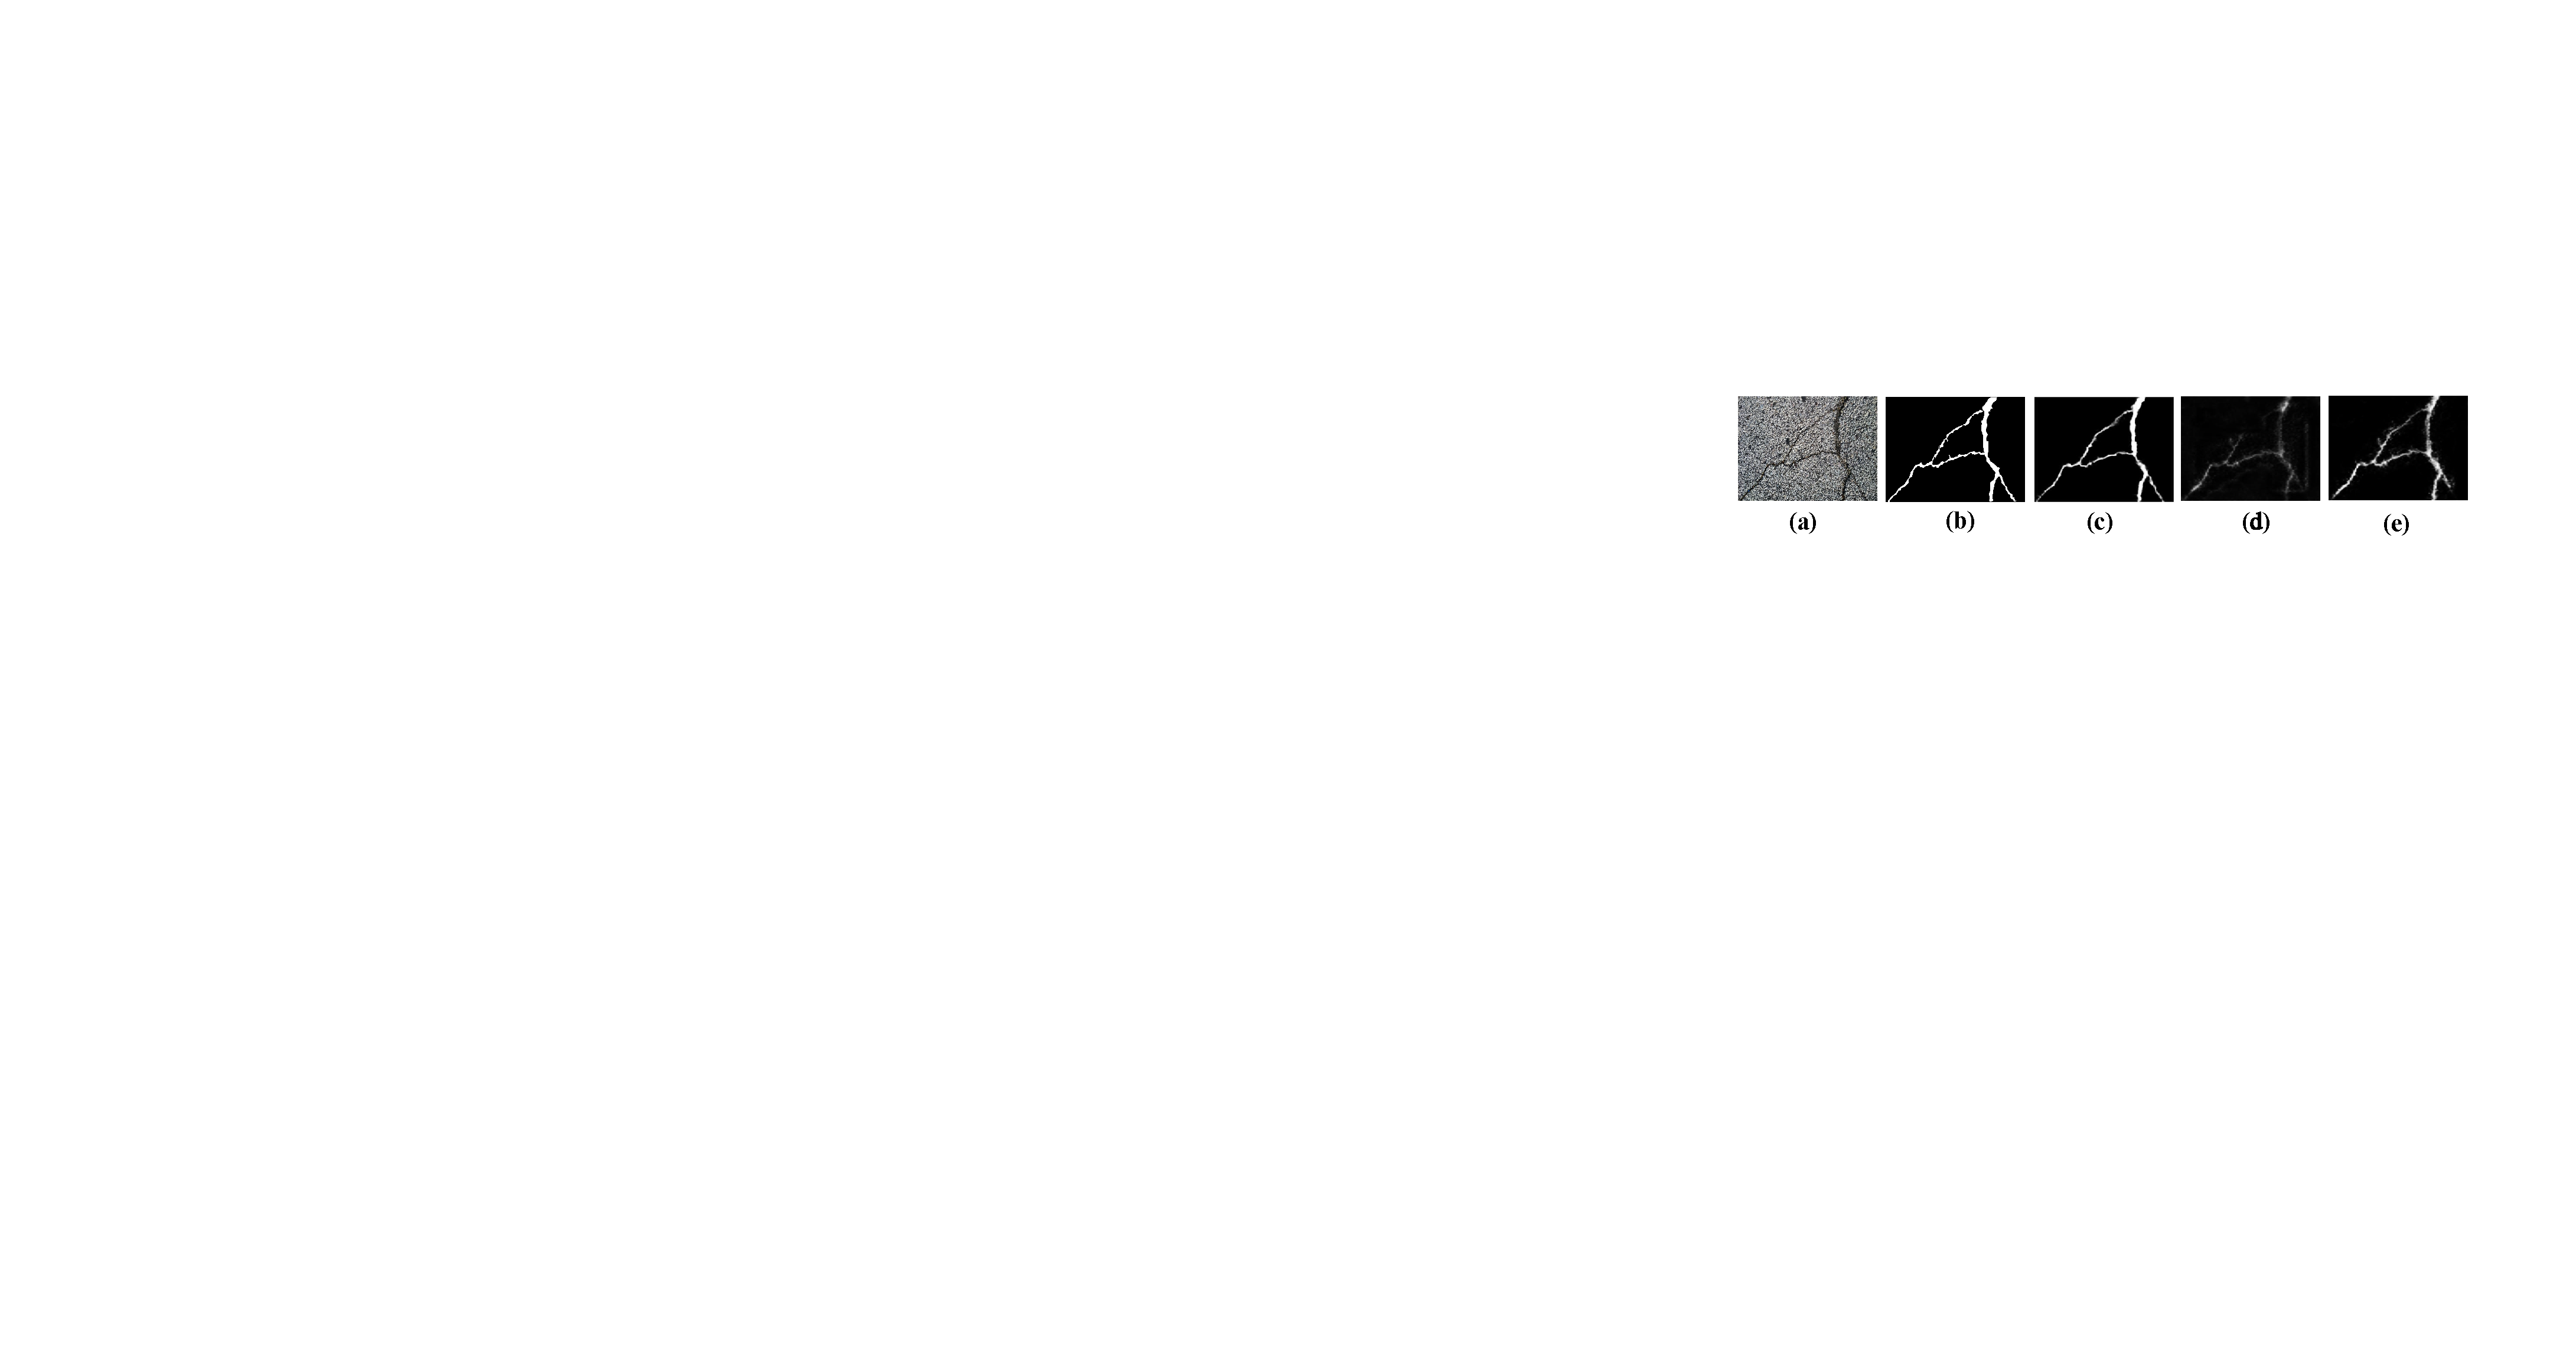
\includegraphics[width=0.95\linewidth]{abl1019.pdf}
\caption{\textcolor{red}{Qualitative comparison of three FAM configurations in Table~II on a purposefully selected
illustrative case from the Crack500 test set.
(a) Input. (b) Ground truth.
(c) Prediction of \emph{Baseline + FAM (Full)}, which fuses the high- and low-frequency branches; per-sample AIU $=$
0.71.
(d) Prediction of \emph{Baseline + FAM (High-Freq)}; per-sample AIU $=$ 0.28.
(e) Prediction of \emph{Baseline + FAM (Low-Freq)}; per-sample AIU $=$ 0.55.
The full-fusion configuration preserves both the main crack contour and the hairline branches, consistent with the quantitative gains in Table~\ref{abla}.}}
\label{ablavis}
\vspace{-0.5cm}
\end{figure}



\textbf{Effectiveness of T-M.} T-M aggregates adjacent frequency-aware levels to produce the coarse localization map used by the refinement stage. Relative to FAM (Full), it improves AIU, AP, and F1 by 0.031, 0.035, and 0.033 on GAPs384 and by 0.034, 0.033, and 0.034 on CFD. The corresponding Crack500 scores decrease by 0.022, 0.019, and 0.017, showing that the benefit of cross-level aggregation is dataset dependent rather than uniform.

\textbf{Effectiveness of HFM.} 
HFM uses the current coarse prediction to guide adjacent-layer fusion. Relative to T-M, it raises all nine accuracy entries by 0.031--0.035 and reduces throughput only from 10.4 to 10.2 FPS. This result supports prior-guided and channel-associated refinement while also quantifying its runtime cost.

In summary, the frequency-guided crack localization step in FANet initially delineates critical areas for potential road cracks, leveraging hierarchical frequency-aware semantic information to highlight these regions. The subsequent detail-preserving crack segmentation step further refines this detection by effectively differentiating the cracks from their surrounding complex background. This refinement is achieved through the integration of high-resolution details, correlation features between adjacent layers, and the initial coarse detection map. Collectively, these stages enable FANet to provide a precise and robust solution for the nuanced task of road crack detection, demonstrating its capacity to navigate the challenges posed by subtle and complex crack patterns within diverse road surfaces.


\subsection{\textcolor{red}{Failure Cases and Limitations}}
\textcolor{red}{Although FANet achieves the best reported accuracy on all five datasets, it still struggles under two identifiable conditions. Fig.~\ref{failurecase} shows two selected failure cases from FANet's predictions. In each column, the top row is the input image, the middle row is the ground truth, and the bottom row is our prediction, so that the gap between the ground truth and our result can be read directly.}

\textcolor{red}{\emph{(1) Fragmentation of low-contrast and camouflaged cracks.} When a crack blends into the pavement and its intensity contrast is low, its frequency evidence can become difficult to distinguish from background texture. A plausible consequence is insufficient support for bridging weak crack segments. As shown in Fig.~\ref{failurecase}(a), the crack that forms a connected structure in the ground truth is broken into disconnected segments in our prediction.}

\textcolor{red}{\emph{(2) Under-segmentation of fine hairline cracks.} When cracks are only a few pixels wide, their frequency evidence can be faint relative to surrounding pavement texture. As shown in Fig.~\ref{failurecase}(b), the thin cracks that are complete in the ground truth are only partially recovered, and some fine branches are missed.}

\textcolor{red}{These observations suggest that the current design is least reliable when crack evidence is not a sufficiently distinct sparse high-frequency signal, particularly at very low contrast or very small width. In addition, two limitations are worth noting. First, the two-step coarse-to-fine pipeline reduces throughput from 13.2 FPS for the PVT baseline to 10.2 FPS for the complete model (22.7\%) on the same hardware, as reported in Table~\ref{abla}. Second, FANet is trained with binary cross-entropy only and imposes no explicit topological continuity constraint, which may contribute to the fragmented predictions above. We plan to explore topology-aware objectives, contrast-adaptive frequency weighting, and complementary sensing modalities such as depth or infrared imaging to push these boundaries in future work.}

\begin{figure}[!ht]
\centering
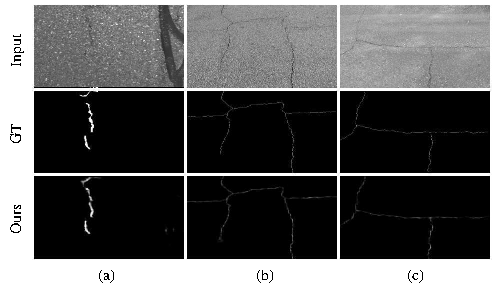
\includegraphics[width=0.79\linewidth,trim=0 0 78.5 0,clip]{failure_cases-1.pdf}
\caption{\textcolor{red}{Representative failure cases of FANet. In each column, the top row is the input image, the middle row is the ground truth, and the bottom row is our prediction. (a) A camouflaged, low-contrast crack whose connected ground-truth structure is fragmented into disconnected segments. (b) A fine hairline crack whose complete ground truth is only partially recovered.}}
\label{failurecase}
\end{figure}

\section{Conclusion}
In this study, we introduce FANet for road crack detection through the joint use of spatial and frequency-domain information. Its frequency-aware module separates and fuses complementary frequency components to generate a coarse crack map, which is then refined through detail-preserving segmentation and a hybrid fusion module. Comparisons on five datasets and module ablations on three datasets demonstrate strong segmentation accuracy while quantifying the associated throughput cost. These results motivate further work on topology-aware objectives and more efficient frequency-spatial modeling for infrastructure inspection.





{\small
\bibliographystyle{IEEEtran}
\bibliography{IEEEfull}
}

\begin{IEEEbiography}[{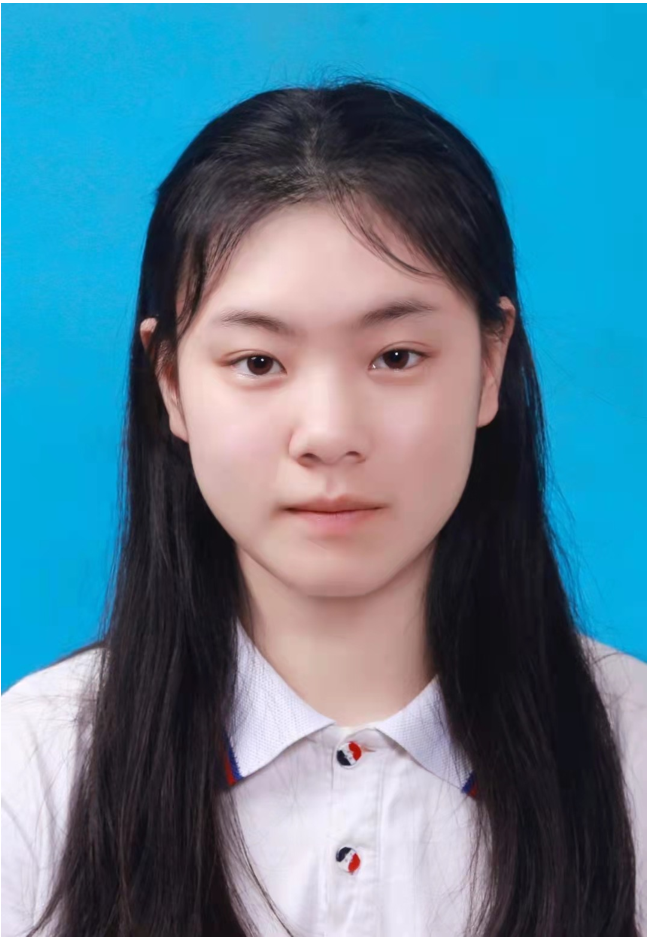
\includegraphics[width=1in,height=1.25in,clip,keepaspectratio]{kuang.pdf}}]{Senyun Kuang} Senyun Kuang received the BSc degree from the School of Information Science and Technology, Southwest Jiaotong University, China, in 2023. She is now pursuing a doctoral degree in the State Key Laboratory of Automotive Safety and Energy, Tsinghua University. She has published 5 papers in CVPR, ICASSP, T-IM, T-IP and T-CSVT. She also has served as a reviewer for T-CSVT, T-IV, T-IM and T-II. Her research interests include computer vision and pattern recognition and intelligent transportation.
\end{IEEEbiography}


\begin{IEEEbiography}[{
\includegraphics[width=1in,height=1.25in,clip,keepaspectratio]{liu.png}}]{Yang Liu} received his Ph.D. degree at Southeast University, China, in 2021. Currently, he is a Marie Curie Fellow and a Research Assistant Professor at the Department of Architecture and Civil Engineering, Chalmers University of Technology, and a Visiting Scholar at the School of Vehicle and Mobility, Tsinghua University. His research interests include intelligent transportation systems, AI techniques, and data mining, with applications in complex real-world problems such as autonomous vehicles and urban mobility. He serves as a Young Editor for two top tier academic journals, including The Innovation and IEEE/CAA Journal of Automatica Sinica. In addition, he is an Associate Editor of IEEE Transactions on Intelligent Vehicles and Journal of Intelligent and Connected Vehicles. Dr. Yang Liu leads a European Union project and a project funded by the Swedish Innovation Agency. He has received numerous awards for his research, including the IEEE ITSM Best Paper High Commendation Award, Honorable Mention of the COTA Best Dissertation Award, ICME Grand Challenge Second Runner-up Award, and the China Highway Society Outstanding Doctoral Dissertation Award. He is experienced in the practice of AI techniques and has won several world prizes in AI competitions organized by leading international AI conferences or research institutes (e.g., KDD, IJCAI, NeurIPS, CVPR, ICME, TRB), including the 1st place of KDD Cup, the most well-known algorithm competition in data mining.
\end{IEEEbiography}






\begin{IEEEbiography}[{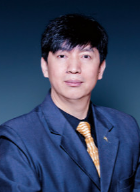
\includegraphics[width=1in,height=1.25in,clip,keepaspectratio]{wyt.png}}]{Yintao Wei} received the B.S. and M.S. degrees in computational mechanics and the Ph.D. degree in composite materials from the Harbin Institute of Technology, Harbin, China, in 1992, 1994, and 1997, respectively. He is currently a tenure Professor with the School of Vehicle and Mobility, Tsinghua University, and the Chair of the Smart Chassis Division. He has managed more than 50 research projects, published more than 100 articles, and awarded more than 30 patents. His research interests include intelligent tires for road perception, smart materials and suspensions, and their industrial applications. He is currently an Associate Editor of the Tire Science and Technology and a reviewer of a number of international journals. 
\end{IEEEbiography}





\begin{IEEEbiography}[{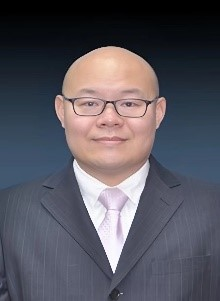
\includegraphics[width=1in,height=1.25in,clip,keepaspectratio]{xiaobo.png}}]{Xiaobo Qu} is a chair professor at the School of Vehicle and Mobility, Tsinghua University, China. He is also an elected Member of Academia Europaea, the Academy of Europe, since August 2020, and a Fellow of the Institution of Engineering and Technology (IET). His research is focused on enhancing urban mobility systems by incorporating emerging technologies, particularly for emergency
services and connected automated vehicles. He has authored or co-authored over 120 journal articles published in top-tier journals, including 14 ESI highly cited papers. He serves as an editor for 10 journals, including the Editor in Chief of Communications in Transportation Research, and Executive Editor in Chief of Journal of Intelligent and Connected Vehicles. To date, Dr. Qu has secured research funding well above 10 million Euros from the Australian Research Council, Swedish Innovation Agency Vinnova, STINT, and the European Union. He has been invited to serve as a panel/assessor for prestigious funding scheme such as the Australian Research Council Centre of Excellence (35 million AUD each), Future Fellowship (career grant, 1 million AUD each), Netherlands NWO VICI (career grant, 2.5 million Euros each), Hong Kong Research Council theme based scheme (30 million HKD each), Singapore Ministry of Education Thematic Research Program (5 million SD each), and the European Research Council, etc.
\end{IEEEbiography}






\end{document}



